\stepcounter{chapter}
\setcounter{eqtn}{0}

\parbf{\ref{ex:ell-infty}.} Check all the conditions in the definition of metric, page \pageref{page:def:metric}.

\parbf{\ref{ex:B2inB1}}; \ref{SHORT.ex:B2inB1:a}.
Observe that $\dist{p}{q}{\spc{X}}\le 1$. 
Apply the triangle inequality to show that $\dist{p}{x}{\spc{X}}\le 2$ for any $x\in B[q,1]$.
Make a conclusion.

\parit{\ref{SHORT.ex:B2inB1:b}.}
Take $\spc{X}$ to be the half-line $[0,\infty)$ with the standard metric; $p=0$ and $q=\tfrac45$.

\parbf{\ref{ex:shrt=>continuous}.}
Show that the conditions in \ref{def:continuous} hold for $\delta=\epsilon$.

\parbf{\ref{ex:close-open}.}
Suppose the complement $\Omega=\spc{X}\backslash Q$ is open.
Then for each point $p\in \Omega$ there is $\epsilon>0$ such that $\dist{p}{q}{\spc{X}}>\epsilon$ for any $q\in Q$.
It follows that $p$ is \emph{not} a limit point of any sequence $q_n\in Q$.
That is, any limit of a sequence in $Q$ lies in $Q$;
by the definition, $Q$ is closed.

Now suppose $\Omega=\spc{X}\backslash Q$ is not open.
Show that there is a point $p\in \Omega$ and a sequence $q_n\in Q$ such that $\dist{p}{q_n}{\spc{X}}\z<\tfrac 1n$ for any~$n$.
Conclude that $q_n\to p$ as $n\to \infty$;
therefore $Q$ is not closed.

\stepcounter{chapter}
\setcounter{eqtn}{0}

\parbf{\ref{ex:9}}; \ref{SHORT.ex:9:compact}. Use that a continuous injection defined on a compact domain is an embedding (\ref{thm:Hausdorff-compact}).

\parit{\ref{SHORT.ex:9:9}.} The image of $\gamma$ might have the shape of the digit $8$ or $9$.

\parbf{\ref{aex:simple-curve}.}
Let $\alpha$ be a path, connecting $p$ to~$q$.

Passing to a subarc of $\alpha$,
we can assume that $\alpha(t)\ne p,q$ for $t\ne0,1$.

An open set $\Omega$ in $(0,1)$ will be called {}\emph{suitable}
if, for any connected component $(a,b)$ of $\Omega$, we have $\alpha(a)=\alpha(b)$.
Show that the union of nested suitable sets is suitable.
Therefore, we can find a maximal suitable set $\hat \Omega$.

Define $\beta(t)=\alpha(a)$ for any $t$ in a connected component $(a,b)\subset\hat \Omega$, and $\beta (t) = \alpha (t) $ for $t\notin\hat{\Omega}$.
Note that for any $x\in [0,1]$ the set $\beta^{-1}\{\beta(x)\}$ is connected.

It remains to show that $\beta$ is a reparametrization of a simple path.
In order to do that, we need to construct a non-decreasing surjective function $\tau\:[0,1]\z\to[0,1]$ such that 
$\tau(t_1)=\tau(t_2)$ if and only if there is a connected component $(a,b)\subset\hat \Omega$ such that $t_1,t_2\z\in [a,b]$.

The required function $\tau$ can be constructed similarly to the so-called {}\emph{devil's staircase} --- learn this construction and modify it.

The simple arc we are looking for is $\beta \circ \sigma$, where $\sigma\: [0,1]\to [0,1]$ is any right inverse of $\tau$.

\parbf{\ref{ex:L-shape}.}
Denote the union of two half-axis by~$L$.

Observe that $f(t)\to\infty$ as $t\to \infty$.
Since $f(0)=0$, the intermediate value theorem implies that $f(t)$ takes all nonnegative values for $t\ge 0$.
Use it to show that $L$ is the range of~$\alpha$.

Further, show that the function $f$ is strictly increasing for $t> 0$.
Use this to show that the map $t\mapsto \alpha(t)$ is injective.

\begin{wrapfigure}[18]{r}{24 mm}
\vskip-4mm
\centering
\includegraphics{mppics/pic-270}
\vskip0mm
\end{wrapfigure}

Summarizing, we get that $\alpha$ is a smooth parametrization of~$L$. 

Now suppose $\beta\:t\mapsto (x(t),y(t))$ is a smooth parametrization of~$L$.
Without loss of generality, we may assume that $x(0)=y(0)=0$.
Note that $x(t)\ge 0$ for any $t$ therefore $x'(0)=0$.
The same way we get that $y'(0)=0$.
That is, $\beta'(0)=0$;
so $L$ does not admit a smooth \emph{regular} parametrization.

\parbf{\ref{ex:cycloid}.}
Apply the definitions.
For \ref{SHORT.ex:cycloid:regular} you need to check that $\gamma'_\ell\ne 0$.
For \ref{SHORT.ex:cycloid:simple} you need to check that $\gamma_\ell(t_0)\z=\gamma(t_1)$ only if $t_0=t_1$.

\parbf{\ref{ex:nonregular}.}
Note that the parametrization $t\mapsto (t,t^3)$ is smooth and regular.
Modify it so it has zero speed at some point.

\parbf{\ref{ex:y^2=x^3}.}
This is the so-called \index{semicubical parabola}\emph{semicubical parabola}; it is shown on the diagram.
Try to argue similarly to \ref{ex:L-shape}.


\parbf{\ref{ex:viviani}.}
For $\ell=0$ the system describes a pair of points $(0,0,\pm1)$, so we can assume that $\ell\ne 0$.
Note that the first equation describes the unit sphere centered at the origin, and the second equation describes a cylinder over the circle in the $(x,y)$-plane with center $(-\tfrac\ell2,0)$ and radius $|\tfrac\ell2|$.


\begin{Figure}
\centering
\vskip-0mm
\begin{lpic}[t(2mm),b(0mm),r(0mm),l(0mm)]{asy/viviani(1)}
\lbl[r]{-.5,13;$x$}
\lbl[l]{31,15;$y$}
\lbl[b]{14,40.5;$z$}
\end{lpic}
\end{Figure}

Find the gradients $\nabla f$ and $\nabla h$ for the functions
\begin{align*}
 f(x,y,z)&=x^2+y^2+z^2-1,
 \\
 h(x,y,z)&=x^2+\ell\cdot x+y^2.
\end{align*}
Show that for $\ell\ne 0$,
the gradients are linearly dependent only on the $x$-axis.
Conclude that for $\ell\ne\pm 1$ each connected component of the set of solutions is a smooth regular curve.

Show that 
\begin{itemize}
\item if $|\ell|<1$, then the set has two connected components with $z>0$ and $z<0$.
\item if $|\ell|\ge1$, then the set is connected.
\end{itemize}

Note that the linear independence of the gradients provides only a sufficient condition.
Therefore, the case $\ell=\pm1$ has to be checked by hand.
In this case, a neighborhood of $(\pm1,0,0)$ does not admit a smooth regular parametrization --- try to prove it. 
The case $\ell=1$ is shown on the diagram.

\parit{Remark.}
In the case $\ell=\pm1$, the curve is called \index{Viviani's curve}\emph{Viviani's curve}.
It admits the following smooth regular parametrization with a self-intersection:
$t\mapsto(\pm(\cos t)^2,\cos t\cdot\sin t,\sin t)$.

\parbf{\ref{ex:open-curve}.}
Assume the contrary, then there is a sequence of real numbers $t_n\to \pm \infty$ such that $\gamma(t_n)$ converges;
denote its limit by~$p$.
Let $K$ be a closed ball centered at~$p$.
Observe that $\gamma^{-1}(K)$ is not compact.
Conclude that $\gamma$ is not proper.



\parbf{\ref{ex:proper-closed}.}
Show and use that a set $C\subset \mathbb{R}^3$ is closed if and only if the intersection $K\cap C$ is compact for any compact $K\subset \mathbb{R}^3$.

\parbf{\ref{ex:proper-curve}.}
Without loss of generality, we may assume that the origin does not lie on the curve.

Show that inversion of the plane $(x,y)\mapsto (\tfrac{x}{x^2+y^2},\tfrac{y}{x^2+y^2})$ maps our curve to a closed curve with the origin removed.
Apply Jordan's theorem for the obtained curve, and use the inversion again.

\stepcounter{chapter}
\setcounter{eqtn}{0}

\parbf{\ref{ex:integral-length-0}.}
Show that if we take the least upper bound in \ref{def:length} for all sequences
$a=t_0\le t_1\le\z\dots\le t_k=b$, then the result is the same.

Suppose $\gamma_2$ is reparametrization of $\gamma_1$ by $\tau\:[a_1,b_1]\to [a_2,b_2]$;
without loss of generality, we may assume that $\tau$ is nondecreasing.
Set $\theta_i=\tau(t_i)$.
Observe that $a_2=\theta_0\z\le\theta_1\le \z\dots\le\theta_k=b_2$ if and only if 
$a_1=t_0\le t_1\le\z\dots\le t_k=b_1$.
Make a conclusion.

\parbf{\ref{ex:length-chain}.}
Show that for any inscribed polygonal line $\beta$ and any $\epsilon>0$ we have
\[\length\beta_n>\length\beta-\epsilon.\]
for all large $n$.
Conclude that
\[\liminf_{n\to\infty}\length\beta_n\ge \length \gamma.\]
Use the definition of length to show that 
\[\limsup_{n\to\infty}\length\beta_n\le \length \gamma.\]
Observe that the two obtained inequalities imply the required statement.

\parbf{\ref{ex:length-image}.}
Choose a partition $0=t_0<\dots <t_n=1$ of $[0,1]$.
Set $\tau_0=0$ and 
\[\tau_i=\max\set{\tau \in[0,1]}{\beta(\tau_i)=\gamma(t_i)}\]
for $i>0$.
Show that $(\tau_i)$ is a partition of $[0,1]$;
that is, $0=\tau_0<\tau_1<\dots<\tau_n=1$.

By construction 
\begin{align*}
|\gamma(t_0)&-\gamma(t_1)|+|\gamma(t_1)-\gamma(t_2)|+\dots
\\
&\qquad\dots+|\gamma(t_{n-1})-\gamma(t_n)|=
\\
&=
|\beta(\tau_0)-\beta(\tau_1)|+|\beta(\tau_1)-\beta(\tau_2)|+\dots
\\
&\qquad\dots+|\beta(\tau_{n-1})-\beta(\tau_n)|.
\end{align*}
Since the partition $(t_i)$ is arbitrary, we get 
\[\length \beta\ge \length \gamma.\]

\parit{Remarks.}
The inequality might be strict.
It happens if $\beta$ runs back and forth along $\gamma$.
In this case the partition $(\tau_i)$ above is \emph{not} arbitrary.

If one assumes only that $\beta([0,1])\supset\gamma([0,1])$, then the problem becomes harder.
It follows from the following useful fact \cite[2.6.1+2.6.2]{burago-burago-ivanov}:
\textit{Denote by $h$ the 1-dimensional Hausdorff measure of the image $\gamma([0,1])$.
Then $h\le \length\gamma$;
moreover the equality holds if $\gamma$ is simple.}

\parbf{\ref{ex:integral-length}.}
For \ref{SHORT.ex:integral-length>}, apply the fundamental theorem of calculus for each segment in a given partition.
For \ref{SHORT.ex:integral-length<} consider a partition such that the velocity vector $\alpha'(t)$ is nearly constant on each of its segments.

\parbf{\ref{adex:integral-length}.}
Use the theorems of Rademacher and Lusin (\ref{thm:rademacher} and \ref{thm:lusin}).

\parbf{\ref{ex:nonrectifiable-curve}}; \ref{SHORT.ex:nonrectifiable-curve:a}.
Look at the diagram, and guess the parametrization of an arc of the snowflake by $[0,1]$.
Extend it to the whole snowflake.
Show that it indeed describes an embedding of the circle into the plane.

\begin{Figure}
\vskip-0mm
\centering
\includegraphics{mppics/pic-226}
\vskip0mm
\end{Figure}

\parit{\ref{SHORT.ex:nonrectifiable-curve:b}.}
Suppose $\gamma\:[0,1]\to\mathbb{R}^2$ is a rectifiable curve and let $\gamma_k$ be a scaled copy of $\gamma$ with factor $k>0$;
that is, $\gamma_k(t)=k\cdot\gamma(t)$ for any~$t$.
Show that 
\[\length\gamma_k=k\cdot\length \gamma.\]

Now suppose the arc $\gamma$ of the Koch snowflake shown on the diagram is rectifiable; denote its length by $\ell$.
Observe that $\gamma$ can be divided into 4 arcs such that each one is a scaled copy of $\gamma$ with factor $\tfrac13$.
It follows that $\ell=\tfrac43\cdot\ell$.
Evidently, $\ell>0$ --- a contradiction.

\parbf{\ref{ex:arc-length-helix}.} 
We have to assume $a\ne 0$ or $b\ne0$;
otherwise, we get a constant curve.

Show that $|\gamma'(t)|\equiv \sqrt{a^2+b^2}$;
in particular, the velocity is constant.
Therefore, $s\z=t/\sqrt{a^2+b^2}$ is an arc-length parameter.
It remains to substitute $s\cdot \sqrt{a^2+b^2}$ for~$t$.




\parbf{\ref{ex:convex-hull}.}
Choose a closed polygonal line $p_1\dots p_n$ inscribed in $\beta$.
By \ref{cor:convex=>rectifiable}, we can assume that its length is arbitrary close to the length of $\beta$;
that is, given $\epsilon>0$ 
\[\length (p_1\dots p_n)>\length\beta-\epsilon.\]

Show that we may assume in addition that each point $p_i$ lies on $\alpha$.

Since $\alpha$ is simple, the points $p_1,\dots,p_n$ appear on $\alpha$ in the same cyclic order;
that is, the polygonal line $p_1\dots p_n$ is also inscribed in $\alpha$.
In particular,
\[\length\alpha\ge \length (p_1\dots p_n).\]
It follows that 
\[\length\alpha>\length\beta-\epsilon.\]
for any $\epsilon>0$.
Whence 
\[\length\alpha\ge\length\beta.\]

\begin{wrapfigure}{r}{25 mm}
\vskip-6mm
\centering
\includegraphics{mppics/pic-275}
\vskip0mm
\end{wrapfigure}

If $\alpha$ has self-intersections, then the points $p_1,\dots, p_n$ might appear on $\alpha$ in a different cyclic order, say $p_{i_1},\dots,p_{i_n}$.
Apply the triangle inequality to show that 
\[\length(p_{i_1}\dots p_{i_n})\ge \length (p_1\dots p_n)\]
and use it to modify the given proof.



\parbf{\ref{ex:convex-croftons}.} 
Denote by $\ell_{\vec u}$ the line segment 
obtained by orthogonal projection of $\gamma$ to the line in the direction ${\vec u}$.
Since $\gamma_{\vec u}$ runs along $\ell_{\vec u}$ back and forth, we get 
\[\length\gamma_{\vec u}\ge 2\cdot\length\ell_{\vec u}.\]
By the Crofton formula, 
\[\length\gamma\ge \pi\cdot \overline{\length\ell_{\vec u}}.\]

In the case of equality, the curve $\gamma_{\vec u}$ runs exactly back and forth along $\ell_{\vec u}$ without additional zigzags for almost all (and therefore for all) ${\vec u}$.

Let $K$ be a closed set bounded by~$\gamma$.
Observe that the last statement implies that every line may intersect $K$ only along a closed segment or a single point.
It follows that $K$ is convex.

\parbf{\ref{adex:more-croftons}.}
The proof is identical to the proof of the standard Crofton formula.
To find the coefficients it is sufficient to check it on a unit interval.
The latter can be done by integration:
\begin{align*}
\frac1{k_a}&=\frac{1}{\area \mathbb{S}^2}\cdot\iint_{\mathbb{S}^2} |x|;
\\
\frac1{k_b}&=\frac{1}{\area \mathbb{S}^2}\cdot\iint_{\mathbb{S}^2} \sqrt{1-x^2}.
\end{align*}
The answers are $k_a=2$ and $k_b=\tfrac4\pi$.

\parbf{\ref{ex:intrinsic-convex}.}
The only-if part is trivial.
To show the if part, assume $A$ is not convex;
that is, there are points $x,y\in A$ and a point $z\notin A$ that lies between $x$ and~$y$.

Since $A$ is closed, its complement is open.
That is, the ball $B(z,\epsilon)$ does not intersect $A$ for some $\epsilon>0$.

Show that there is $\delta>0$ such that any path of length at most $\dist{x}{y}{\mathbb{R}^3}+\delta$ passes thru $B(z,\epsilon)$.
It follows that $\dist{x}{y}A\ge \dist{x}{y}{\mathbb{R}^3}+\delta$; 
in particular, $\dist{x}{y}A\ne \dist{x}{y}{\mathbb{R}^3}$.

\begin{wrapfigure}{r}{30 mm}
\vskip-0mm
\centering
\includegraphics{mppics/pic-280}
\vskip0mm
\end{wrapfigure}

\parbf{\ref{ex:antipodal}.}
The spherical curve shown on the diagram does not have antipodal pairs of points.
However, it has three points $x,y,z$ on one of its sides and their antipodal points $-x,-y,-z$ on the other.
Show that this property is sufficient to conclude that the curve does not lie in any hemisphere.

\parbf{\ref{ex:bisection-of-S2}.}
Assume the contrary, then by the hemisphere lemma (\ref{lem:hemisphere}) $\gamma$ lies in an open hemisphere.
In particular, it cannot divide $\mathbb{S}^2$ into two regions of equal area --- a contradiction.

\parbf{\ref{ex:flaw}.}
The very first sentence is wrong --- it is {}\emph{not} sufficient to show that the diameter is at most~2.
For example, if an equilateral triangle has circumradius slightly above $1$,
then its diameter (which is defined as the maximal distance between its points) is slightly bigger than $\sqrt3$, so it is smaller than $2$.

On the other hand, it is easy to modify the proof of the hemisphere lemma (\ref{lem:hemisphere}) to get a correct solution.
That is, (1) choose two points $p$ and $q$ on $\gamma$ that divide it into two arcs of the same length;
(2) set $z$ to be a midpoint of $p$ and $q$,
and (3) show that $\gamma$ lies in the unit disc centered at~$z$.


\parbf{\ref{adex:crofton}.}
For \ref{SHORT.adex:crofton:crofton}, modify the proof of the original Crofton formula
(Section~\ref{sec:crofton}).

\parit{\ref{SHORT.adex:crofton:hemisphere}.}
Assume $\length \gamma<2\cdot\pi$.
By \ref{SHORT.adex:crofton:crofton},
\[\overline{\length \gamma^*_{\vec u}}<2\cdot\pi.\]
Therefore, we can choose ${\vec u}$ so that 
\[\length \gamma^*_{\vec u}<2\cdot\pi.\]

Observe that $\gamma^*_{\vec u}$ runs in a semicircle~$h$.
Therefore $\gamma$ lies in a hemisphere with $h$ as a diameter.

\stepcounter{chapter}
\setcounter{eqtn}{0}


\parbf{\ref{ex:zero-curvature-curve}.}
For a unit-speed parametrization $\gamma$, we have $\gamma''\equiv 0$.
Therefore, the velocity $\vec v=\gamma'$ is constant.
Hence, $\gamma(t)=p+(t-t_0)\cdot \vec v$, where $p=\gamma(t_0)$.


\parbf{\ref{ex:scaled-curvature}.} 
Observe that $\alpha(t)\df\gamma_{\lambda}(t/\lambda)$ is a unit-speed parametrization of the curve $ \gamma_{\lambda}$.
Apply the chain rule twice.


\parbf{\ref{ex:curvature-of-spherical-curve}.} Differentiate the identity $\langle\gamma(s),\gamma(s)\rangle=1$ a couple of times.

\parbf{\ref{ex:curvature-formulas}.} 
Set $\tan=\tfrac{\gamma'}{|\gamma|}$.
Prove and use the following identities: 
\begin{align*}
\gamma''-(\gamma'')^\perp&=\tan\cdot\langle\gamma'',\tan\rangle,
&
|\gamma'|&=\sqrt{\langle \gamma',\gamma'\rangle}.
\end{align*}

\parbf{\ref{ex:curvature-graph}.} 
Apply \ref{ex:curvature-formulas:a} for the parametrization $t\z\mapsto (t,f(t))$.

\parbf{\ref{ex:approximation-const-curvature}.}
Without loss of generality, we may assume that $\gamma$ has a unit-speed parametrization.

Consider the tangent indicatrix $\tan(s)=\gamma'(s)$.
Note that $\tan$ is a spherical curve and $|\tan'|\le 1$.
Use it to construct a sequence of unit-speed spherical curves $\tan_n\:\mathbb{I}\to\mathbb{S}^2$ such that $\tan_n(s)\to \tan(s)$ as $n\to\infty$ for any~$s$.
Show that the following sequence of curves solves the problem:
\[\gamma_n(s)=\gamma(a)+\int_a^s\tan_n(t)\cdot dt.\]

\parbf{\ref{ex:no-parallel-tangents}.}
Reuse the construction in \ref{ex:antipodal} to get a closed smooth simple spherical curve $\tan\:\mathbb{S}^1\z\to\mathbb{S}^2$ that contains no pair of antipodal points and has zero average.
Then construct a curve with tangent indicatrix $\tan$.
(It was constructed by Beniamino Segre \cite{segre}.)

\parbf{\ref{ex:helix-curvature}.}
Show that $\gamma_{a,b}''\perp \gamma'_{a,b}$, and apply \ref{ex:curvature-formulas:a}.

\parbf{\ref{ex:length>=2pi}.} Apply Fenchel's theorem.

\parbf{\ref{ex:gamma/|gamma|}.}
We can assume that $\gamma$ is unit-speed.
Set $\theta(s)=\measuredangle(\gamma(s),\gamma'(s))$.
Since $\langle\tan,\tan\rangle=1$, we have $\tan'\perp \tan$.
Observe that $\langle \tan,\sigma\rangle=\cos\theta$;
therefore
\begin{align*}
\kur\cdot \sin\theta
&=|\tan'|\cdot \sin\theta\ge
-\langle \tan',\sigma\rangle=
\\
&=
\langle \tan,\sigma'\rangle-\langle \tan,\sigma\rangle'=
\\
&=
(|\sigma'|+\theta')\cdot \sin\theta.
\end{align*}
Whence $\kur\ge |\sigma'|+\theta'$
if $\theta\ne0,\pi$.
It remains to integrate this inequality and show that the set with $\theta\ne0$ or $\pi$ does not create a problem.

\parit{An alternative solution} can be built on \ref{prop:inscribed-total-curvature}.

\parbf{\ref{ex:DNA}}; \ref{SHORT.ex:DNA:c''c>=k}.
Since $|\gamma(s)|\le 1$, we have
\begin{align*}
\langle\gamma''(s),\gamma(s)\rangle&\ge -|\gamma''(s)|\cdot|\gamma(s)|\ge-\kur(s)
\end{align*}
for all~$s$.

\parit{\ref{SHORT.ex:DNA:int>=length-tc}.}
Since $\gamma$ is unit-speed, we have $\ell=\length\gamma$ and $\langle\gamma',\gamma'\rangle\equiv1$.
Therefore,
\begin{align*}
\int_0^\ell\langle\gamma(s),\gamma'(s)\rangle'\cdot ds
&=
\int_0^\ell\langle\gamma'(s),\gamma'(s)\rangle\cdot ds+
\\
&+\int_0^\ell\langle\gamma(s),\gamma''(s)\rangle\cdot ds\ge
\\
&\ge \length\gamma-\tc\gamma.
\end{align*}

\parit{\ref{SHORT.ex:DNA:end}.}
By the fundamental theorem of calculus, we have
\begin{align*}
\int_0^\ell\langle\gamma(s),\gamma'(s)\rangle'\cdot ds
&=\langle\gamma(\ell),\gamma'(\ell)\rangle
-
\langle\gamma(0),\gamma'(0)\rangle.
\end{align*}
Since $\gamma(0)=\gamma(\ell)$ and $\gamma'(0)=\gamma'(\ell)$, the right-hand side vanishes.


Note that without loss of generality, we can assume the curve in \ref{thm:DNA} is described by a loop $\gamma\:[0,\ell]\to\mathbb{R}^3$ parametrized by arc-length.
We can also assume that the origin is the center of the ball; that is $|\gamma|\le 1$.
Since $\gamma$ is a smooth closed curve, we have 
$\gamma'(0)=\gamma'(\ell)$ and $\gamma(0)=\gamma(\ell)$.
Therefore, \ref{SHORT.ex:DNA:int>=length-tc} and \ref{SHORT.ex:DNA:end} imply \ref{thm:DNA}.

\parbf{\ref{ex:tangent-support}.}
Show that no line distinct from $\ell$ can support $F$ at $p$. 
Apply \ref{lem:separation} to show that there is a line supporting $F$ at $p$.
Conclude that it must be $\ell$.

{

\begin{wrapfigure}{r}{22 mm}
\vskip-6mm
\centering
\includegraphics{mppics/pic-255}
\vskip0mm
\end{wrapfigure}

\parbf{\ref{ex:anti-bow}.}
Start with the curve $\gamma_1$ shown on the diagram.
To obtain $\gamma_2$, slightly unbend (that is, decrease the curvature of) the dashed arc of $\gamma_1$.


\parbf{\ref{ex:length-dist}}; \ref{SHORT.ex:length-dist:>}.
Choose a value $s_0\in[a,b]$ that splits the total curvature of $\gamma$ into two equal parts.
Observe that $\measuredangle(\gamma'(s_0),\gamma'(s))\le \theta$ for any~$s$.
Use this inequality in the same way as in the proof of the bow lemma.

Part \ref{SHORT.ex:length-dist:sef-intersection:>pi} is straightforward.
For part \ref{SHORT.ex:length-dist:=} consider the the concatenation of two equal line segment with the external angle $2\cdot\theta$ and smooth its joint. 


}

\parbf{\ref{ex:schwartz}.}
Let $\ell=\length\gamma$.
Suppose $\ell_1<\ell<\ell_2$.
Let $\gamma_1$ be an arc of unit circle with length $\ell$.

Show that the distance between the endpoints of $\gamma_1$ is smaller than $|p-q|$, and apply the bow lemma (\ref{lem:bow}).


\parbf{\ref{ex:loop}.}
Suppose $\length\gamma<2\cdot\pi$. 
Apply the bow lemma (\ref{lem:bow}) to $\gamma$ and an arc of the unit circle of the same length.

\parbf{\ref{ex:bow-upper}.}
Choose a smooth regular spherical curve $\alpha$ that runs near one point;
for example, a small spherical circle centered at this point.
Consider a curve $\tan$ that runs along $\alpha$ with speed $\kappa(s)$ at any $s\in [0,\ell]$.
Show that a curve with tangent indicatrix $\tan$ solves the problem.

\parbf{\ref{ex:chord-lemma-optimal}.} 
Set $\alpha=\measuredangle(\vec w,\vec u)$ 
and $\beta=\measuredangle(\vec v,\vec u)$.
Try to guess the example from the diagram.

\begin{Figure}
\vskip-0mm
\centering
\includegraphics{mppics/pic-285}
\vskip0mm
\end{Figure}

The shown curve is divided into three arcs: I, II, and III. 
Arc I turns from $\vec v$ to $\vec u$;
it has total curvature $\alpha$.
Similarly, arc III turns from $\vec u$ to $\vec w$ and has total curvature $\beta$. 
Arc II goes very close and almost parallel to the chord $pq$, and its total curvature can be made arbitrarily small.


\parbf{\ref{ex:monotonic-tc}.}
Use the fact that an exterior angle of a triangle equals the sum of the two remote interior angles.
For the second part apply induction on the number of vertices.

\parbf{\ref{ex:total-curvature=}.}
By \ref{prop:inscribed-total-curvature}, $\tc\gamma\ge \tc\beta$;
it remains to show that
$\tc\gamma\le\sup\{\tc\beta\}$.
In other words, 
given $\epsilon>0$ and a polygonal line $\sigma=\vec u_0\dots \vec u_k$ inscribed in the tangent indicatrix $\tan$ of $\gamma$, 
we need to construct a polygonal line $\beta$ inscribed in $\gamma$ such that
\[\length\sigma<\tc\beta+\epsilon.
\eqlbl{eq:tc=<tc}\]

Suppose $\vec u_i=\tan(s_i)$.
Choose an inscribed polygonal line $\beta=p_0\dots p_{2\cdot k+1}$ such that $p_{2\cdot i}$ and $p_{2\cdot i+1}$ lie sufficiency close to $\gamma(s_i)$; so we can assume that the direction of $p_{2\cdot i+1}-p_{2\cdot i}$ is sufficiency close to $\vec u_i$ for each~$i$.
Show that \ref{eq:tc=<tc} holds true for the constructed polygonal line $\beta$.

\begin{wrapfigure}{r}{23 mm}
\vskip-3mm
\centering
\includegraphics{mppics/pic-290}
\vskip-0mm
\end{wrapfigure}

\parbf{\ref{ex:sef-intersection}}; \ref{SHORT.ex:sef-intersection:<2pi} See the diagram. 

\parit{\ref{SHORT.ex:sef-intersection:>pi}.} Assume $x$ is a point of self-intersection.
Show that we may choose two points $y$ and $z$ on $\gamma$ so that the triangle $xyz$ is nondegenerate.
In particular, 
$\measuredangle\hinge yxz
\z+
\measuredangle\hinge zyx
<\pi$, or, equivalently, for the \emph{nonclosed} polygonal line $xyzx$ we have $\tc{xyzx}>\pi$.
It remains to apply \ref{prop:inscribed-total-curvature}.

\parbf{\ref{ex:quadrisecant}.}
Consider the closed polygonal line $acbd$.
Observe that $\tc{acbd}=4\cdot\pi$.
It remains to apply \ref{prop:inscribed-total-curvature}.

\parbf{\ref{ex:tc-rectifiable}.} Observe that $\gamma$ lies in a ball of finite radius and apply \ref{thm:DNA-poly} for its rescaling.

\stepcounter{chapter}
\setcounter{eqtn}{0}

{

\begin{wrapfigure}{r}{12 mm}
\vskip-3mm
\centering
\begin{lpic}[t(-0mm),b(0mm),r(0mm),l(0mm)]{asy/helix(1)}
\lbl[br]{8,24;$\norm$}
\lbl[b]{2,26;$\bi$}
\lbl[wl]{15,25;$\tan$}
\end{lpic}
\vskip-0mm
\end{wrapfigure}

\parbf{\ref{ex:helix-torsion}.} 
The arc-length parameter $s$ is already found in   \ref{ex:arc-length-helix}.
It remains to find the Frenet frame and calculate curvature and torsion.
The latter can be done by straightforward calculations;
the answers are 
\begin{align*}
\tan(t)&=\tfrac{1}{\sqrt{a^2+b^2}}\cdot(-a\cdot\sin t, a\cdot\cos t,b),
\\
\norm(t)&=(-\cos t,-\sin t,0),
\\
\bi(t)&=\tfrac{1}{\sqrt{a^2+b^2}}\cdot(b\cdot \sin t,-b\cdot \cos t, a),
\\
\kur &\equiv \tfrac{a}{a^2+b^2},\qquad
\tor \equiv \tfrac{b}{a^2+b^2}.
\end{align*}

It remains to show that the map $(a,b) \mapsto (\frac{a}{a^2+b^2}, \frac{b}{a^2+b^2})$ sends bijectively the half plane $a>0$ onto itself.

}

\parbf{\ref{ex:beta-from-tau+nu}.} By the product rule, we get
\begin{align*}
\bi'&=(\tan\times \norm)'=
\tan'\times \norm+\tan\times\norm'.
\end{align*}
It remains to substitute the values from \ref{eq:frenet-tau} and \ref{eq:frenet-nu} and simplify.

\parbf{\ref{ex:torsion=0}.}
This is a consequence of the equation $\bi' = - \tor\cdot \norm $.

\parbf{\ref{ex:frenet}.}
Observe that $\tfrac{\gamma'\times\gamma''}{|\gamma'\times\gamma''|}$ is a unit vector perpendicular to the plane spanned by $\gamma'$ and $\gamma''$, so, up to sign, it has to be equal to $\bi$.
It remains to check that the sign is right.

\parbf{\ref{ex:torsion-indicatrix}.} Assume that tangent indicatrix has no self-intersection.
Show that it lies in an open hemisphere and argue as in Fenchel's theorem.

\parbf{\ref{ex:lancret}}; \ref{SHORT.ex:lancret:a}.
Observe that 
$\langle \vec w,\tan\rangle'=0$.
Show that it implies that $\langle \vec w, \norm\rangle =0$.

By Frenet formulas,  
$\langle \vec w,\norm\rangle'=0$
 implies 
$\langle \vec w, -\kur\cdot\tan+\tor\cdot \bi\rangle =0$.

\parit{\ref{SHORT.ex:lancret:b}.}
Show that $\vec w'=0$;
it implies that $\langle \vec w,\tan\rangle=\tfrac\tor\kur$.
In particular, the velocity vector of $\gamma$ makes a constant angle with $\vec w$; that is, $\gamma$ has a constant slope.

\parbf{\ref{ex:evolvent-constant-slope}.}
Suppose $\alpha$ is an evolvent of $\gamma$, and $\vec w$ is a fixed vector.
Show that $\langle \vec w,\alpha\rangle$ is constant if $\gamma$ makes a constant angle with $\vec w$.

\parbf{\ref{ex:spherical-frenet}}.
Part \ref{SHORT.ex:spherical-frenet:tau} follows from the fact that $(  \tan,\norm,\bi)$ is an orthonormal basis.
For \ref{SHORT.ex:spherical-frenet:nu} take the first and second derivatives of the identity $\langle\gamma,\gamma\rangle=1$ and simplify using the Frenet formulas.
Part \ref{SHORT.ex:spherical-frenet:beta} follows from \ref{SHORT.ex:spherical-frenet:nu} and the Frenet formulas.
By \ref{SHORT.ex:spherical-frenet:beta}, $\int\tfrac\tor\kur=0$, hence \ref{SHORT.ex:spherical-frenet:beta+} follows.
Part \ref{SHORT.ex:spherical-frenet:kur-tor} is proved by algebraic manipulations.

\parit{\ref{SHORT.ex:spherical-frenet:f}.}
Use the Frenet formulas to show that $(\gamma+\tfrac1\kur\cdot \norm+\tfrac{\kur'}{\kur^2\cdot\tor}\cdot\bi)'=0$.



\parbf{\ref{ex:cur+tor=helix}.} Use the second statement in \ref{ex:helix-torsion}.

\parbf{\ref{ex:const-dist}.} Note that the function
\begin{align*}
\rho(\ell)&=|\gamma(t+\ell)-\gamma(t)|^2=
\\
&=\langle \gamma(t+\ell)-\gamma(t),\gamma(t+\ell)-\gamma(t)\rangle
\end{align*}
is smooth and does not depend on~$t$.
Express speed, curvature, and torsion of $\gamma$ in terms of the derivatives $\rho^{(n)}(0)$.
Be patient, you will need two derivatives for the speed,
four for the curvature,
and six for the torsion.
Once it is done, apply \ref{ex:cur+tor=helix}.

\stepcounter{chapter}
\setcounter{eqtn}{0}



\parbf{\ref{ex:bike}.}
Without loss of generality, we may assume that $\gamma_0$ is parametrized by its arc-length.
Then
\begin{align*}
|\gamma_1'|&=|\gamma_0'+\tan'|=|\tan+\kur\cdot\norm|
=
\\
&=
\sqrt{1+\kur^2}
\ge
1=
|\gamma_0'|;
\end{align*}
that is, $|\gamma_1'(t)|\ge|\gamma_0'(t)|$ for any $t\in[a,b]$.
Integrate this inequality and apply 
\ref{ex:integral-length}.


\parbf{\ref{ex:trochoids}.}
Observe that $\gamma'_a(t)=(1+a\cdot \cos t, -a\cdot \sin t)$;
that is, $\gamma'_a$ runs clockwise along a circle with center at $(1,0)$ and radius $\vert a \vert$.

\parit{Case $|a|>1$.} Note that $\tan_a(t)=\gamma'_a/|\gamma'_a|$ runs clockwise and makes a full turn in time $2\cdot\pi$.
Therefore, $\tgc{\gamma_a}=-2\cdot\pi$ and $\tc\gamma_a=|\tgc{\gamma_a}|=2\cdot\pi$.

\parit{Case $|a|<1$.}
Set $\theta_a=\arcsin a$.
Show that $\tan_a(t)=\gamma'_a/|\gamma'_a|$ starts with the horizontal direction $\tan_a(0)=(1,0)$, turns monotonically to angle $\theta_a$, then monotonically to $-\theta_a$ and then monotonically back to $\tan_a(2\cdot\pi)=(1,0)$.
It follows that if $|a|>1$, then
$\tgc{\gamma_a}=0$ and $\tc{\gamma_a}=4\cdot\theta_a$.

\parit{Case $a=-1$.}
The velocity $\gamma'_{-1}(t)$ vanishes at $t=0$ and $2\cdot\pi$.
Nevertheless, the curve admits a smooth regular parametrization --- find it.
The answer is $\tc{\gamma_{-1}}=-\tgc{\gamma_{-1}}=\pi$.

\parit{Case $a=1$.}
The velocity $\gamma'_1(t)$ vanishes at $t=\pi$.
At $t=\pi$ the curve has a cusp;
that is, $\gamma_1$ turns exactly back at the time $\pi$.
So $\gamma_1(t)$ has undefined total signed curvature.
The curve is a joint of two smooth arcs with external angle $\pi$, and
the total curvature of each arc is $\tfrac\pi2$, so 
$\tc{\gamma_{1}}=\tfrac\pi2+\pi+\tfrac\pi2=2\cdot\pi$.


\parbf{\ref{ex:zero-tsc}.}
The answers are shown.
In the last picture, we assume that the two marked points have parallel tangent lines.

\begin{Figure}
\begin{minipage}{.32\textwidth}
\centering
\includegraphics{mppics/pic-260}
\end{minipage}\hfill
\begin{minipage}{.32\textwidth}
\centering
\includegraphics{mppics/pic-261}
\end{minipage}
\hfill
\begin{minipage}{.32\textwidth}
\centering
\includegraphics{mppics/pic-262}
\end{minipage}
\end{Figure}

\parbf{\ref{ex:length'}}; \ref{SHORT.ex:length':reg}.
Show that
\[
\gamma_\ell'(t)=(1-\ell\cdot\skur(t))\cdot \gamma'(t).
\]
By regularity of $\gamma$, $\gamma'\ne0$.
So if $\gamma_\ell'(t)=0$, then $\ell\cdot \skur(t)= 1$.

\parit{\ref{SHORT.ex:length':formula}.} We can assume that $\gamma$ is parametrized by its arc-length, so $\gamma'(t)=\tan(t)$.
Suppose $|\ell|<\frac{1}{\kur(t)}$ for any~$t$.
Then 
\[
|\gamma_\ell'(t)|=(1-\ell\cdot\skur(t)).
\]
Therefore,
\begin{align*}
L(\ell)
&=
\int_a^b(1-\ell\cdot\skur(t))\cdot dt=
\\&=
\int_a^b 1\cdot dt-\ell\cdot \int_a^b\skur(t)\cdot dt=
\\
&=
L(0)+\ell\cdot\tgc\gamma.
\end{align*}



\parit{\ref{SHORT.ex:length':antiformula}.}
Consider the unit circle $\gamma(t)=(\cos t,\sin t)$ for $t\in[0,2\cdot\pi]$ and $\gamma_\ell$ for $\ell=2$.

\parbf{\ref{ex:inverse}.}
Use the definition of osculating circle via order of contact, plus use the fact that inversions send circles to circlines. 

\parbf{\ref{ex:evolute-of-ellipse}.}
Find $\tan(t)$ and $\norm(t)$.
Use the formula in \ref{ex:curvature-formulas:b} to calculate curvature $\kur(t)$.
Apply the formula given right before the exercise.

\begin{wrapfigure}{r}{15 mm}
\vskip-4mm
\centering
\includegraphics{mppics/pic-296}
\vskip-3mm
\end{wrapfigure}

\parbf{\ref{ex:3D-spiral}.}
Start with a plane spiral curve as shown on the diagram.
Applying \ref{thm:fund-curves}, increase the torsion of the dashed arc without changing the curvature until a self-intersection appears.
You may think that the dashed arc is very short, so the tangent vector $\tan$ is nearly constant on this arc. 
Note that increasing the torsion can rotate normal vector $\norm$ arbitrary around $\tan$.
An intersection appears if $\norm$ is rotated by certain angle near $\pi$.
(Compare to \ref{ex:approximation-const-curvature}.)

\parbf{\ref{ex:double-tangent}.} 
Observe that if a line or circle is tangent to $\gamma$,
then it is tangent to the osculating circle at the same point.
Then apply the spiral lemma (\ref{lem:spiral}).

\parbf{\ref{ex:spherical-spiral}.}
Note that osculating circles of a spherical curve lie in the sphere.
Prove an analog of \ref{lem:spiral} for these circles.
(Compare to \ref{ex:spherical-frenet:beta+}.)

\stepcounter{chapter}
\setcounter{eqtn}{0}

\parbf{\ref{ex:vertex-support}.}
Apply the spiral lemma (\ref{lem:spiral}).

\parit{Computational solution.} 
We will assume that the curvature does not vanish at $p$, the remaining case is simpler.
We may assume that $\gamma$ is unit-speed, $p=\gamma(0)$,
and the center of curvature of $\gamma$ at $p$ is the origin;
in other words, $\kur(0)\cdot\gamma(0)+ \norm(0)=0$.

Consider the function $f\:t\mapsto \langle\gamma(t),\gamma(t)\rangle$.
Direct calculations show that 
\begin{align*}
f'
&=\langle\gamma,\gamma\rangle'
=2\cdot\langle\tan,\gamma\rangle,
\\
f''
&=2\cdot\langle\tan,\gamma\rangle'
=2\cdot\kur\cdot\langle\norm,\gamma\rangle+2,
\\
f'''
&=2\cdot\kur'\cdot\langle\norm,\gamma\rangle
+2\cdot\kur\cdot\langle\norm',\gamma\rangle+\cancel{2\cdot\kur\cdot\langle\norm,\tan\rangle}.
\end{align*}

Observe that $\norm'(0)\perp\gamma(0)$.
Therefore, $f'(0)=0$, $f''(0)=0$, and $f'''(0)\z=-2\cdot\kur'/\kur$.

If the osculating circle supports $\gamma$ at $p$,
then the function $f$ has a local maximum or minimum at $0$.
Therefore $f'''(0)=0$ and $\kur'=0$.

\parbf{\ref{ex:support}.}
Consider the coordinate system with the origin at $p$ and the common tangent line to $\gamma_1$ and $\gamma_2$ as the $x$-axis.
We may assume that $\gamma_1$ and $\gamma_2$ are defined in $(-\epsilon,\epsilon)$ for some small $\epsilon>0$,
so that they run almost horizontally.

Given $t\in[0,1]$ consider the curve $\gamma_t$ that is tangent and cooriented to the $x$-axis at $\gamma_t(0)$ and has signed curvature defined by $\skur_t(s)\df(1\z-t)\cdot\skur_0(s)+t\cdot\skur_1(s)$.
It exists by \ref{thm:fund-curves-2D}.

Choose $s\approx 0$.
Consider the curve $\alpha_s\:t\mapsto \gamma_t(s)$.
Show that $\alpha_s$ moves almost vertically up.
Use the fact that $\gamma_t$ moves almost horizontally to show that in a small neighborhood of $p$, the curve $\gamma_1$ lies above $\gamma_0$,
whence the statement follows.

\parbf{\ref{ex:in-circle}.} Move the center of the unit circle to the base of the loop and then reduce its radius to zero.
Show that at the moment when the circle first touch the loop, it supports the loop at a point distinct from the base.
Apply \ref{prop:supporting-circline}.


\parbf{\ref{ex:between-parallels-1} $\bm{+}$ \ref{ex:in-triangle} $\bm{+}$ \ref{ex:lens}.}
Observe that one of the arcs of curvature 1 in the families shown on the diagram supports $\gamma$, and apply \ref{prop:supporting-circline}.

\begin{Figure}
\begin{minipage}{.50\textwidth}
\centering
\includegraphics{mppics/pic-265}
\end{minipage}\hfill
\begin{minipage}{.26\textwidth}
\centering
\includegraphics{mppics/pic-266}
\end{minipage}
\hfill
\begin{minipage}{.20\textwidth}
\centering
\includegraphics{mppics/pic-267}
\end{minipage}
\end{Figure}
The second part in \ref{ex:between-parallels-1} can be reduced to \ref{ex:in-circle} using the shown family and another family of arcs curved in the opposite direction.

\parit{Remark.} Compare to \ref{ex:moon-rad}.

\begin{wrapfigure}{r}{34 mm}
\vskip-8mm
\centering
\includegraphics{mppics/pic-268}
\vskip0mm
\end{wrapfigure}

\parbf{\ref{ex:convex small}.}
Note that we can assume that $\gamma$ bounds a convex figure~$F$. Otherwise, by \ref{prop:convex} its curvature changes sign.
Therefore, $\gamma$ has zero curvature at some point.

Choose two points $x$ and $y$ surrounded by $\gamma$ such that $|x\z-y|\z>2$.
Look at the maximal lens bounded by two arcs with a common chord $xy$ that lies in~$F$.
Apply the supporting test (\ref{prop:supporting-circline}).

\parbf{\ref{ex:line-curve-intersections}}; \ref{SHORT.ex:line-curve-intersections:a}.
Apply the lens lemma to show that if $p_2$ lies between $p_1$ and $p_3$, then the curvature of $\gamma$ switches its sign.

\parit{\ref{SHORT.ex:line-curve-intersections:b}.} Show that $p_4$ lies between $p_2$ and $p_3$;
further $p_5$ lies between $p_3$ and $p_4$;
and so on.

\parit{\ref{SHORT.ex:line-curve-intersections:c}.}
According to \ref{SHORT.ex:line-curve-intersections:a}, the point $p_3$ might lie between $p_1$ and $p_2$, and then further order is determined uniquely, or $p_1$ lies between $p_2$ and $p_3$.
In the latter case, we have two choices, either $p_4$ lies between $p_2$ and $p_3$, and then further order is determined uniquely, or $p_2$ lies between $p_3$ and $p_4$.
In the latter case, we get a choice again.

\begin{Figure}
\vskip-0mm
\centering
\includegraphics{mppics/pic-29}
\vskip0mm
\end{Figure}

Assume we make the first choice on the step number~$k$.
Without loss of generality, we may assume that $p_k$ lies to the right from $p_{k-2}$.
Then we have the following order:
\[
p_{k-2},p_{p-4},\dots,p_{p-5},p_{k-3},p_k,p_{k+2},\dots,p_{k+1},p_{k-1}.
\]
The case $k=7$ and $n=11$ is shown on the diagram.

\parbf{\ref{ex:moon-rad}.}
Show that $\gamma$ contains a simple loop $\gamma_1$.
Apply to $\gamma_1$ \ref{thm:moon-orginal}.

\parbf{\ref{ex:moon-area}.} 
Applying scaling, we may assume that $a=\pi$; that is, $\gamma$ bounds area of the unit disc.
Then apply \ref{thm:moon} to show that the curvature is at least 1 at some point.
Argue as at the end of the proof of \ref{thm:4-vert-supporting}, showing that the curvature is at most 1 at some point.
Apply the intermediate value theorem to show that curvature is  1 at some point.

\begin{wrapfigure}{r}{25 mm}
\vskip-4mm
\centering
\includegraphics{mppics/pic-305}
\vskip0mm
\end{wrapfigure}

\parbf{\ref{ex:curve-crosses-circle}.}
Repeat the proof of the \ref{thm:moon} for each cyclic concatenation of an arc of $\gamma$ from $p_i$ to $p_{i+1}$ with a large arc of the circle. 

An example for the second part can be guessed from the diagram.

\stepcounter{chapter}
\setcounter{eqtn}{0}

\parbf{\ref{ex:hyperboloids}.} 
Denote the level set by $\Sigma_\ell$.

Show that $\nabla_p f=0$ if and only if $p=(0,0,0)$.
Use \ref{prop:implicit-surface} to conclude that if $\ell\ne 0$, then $\Sigma_\ell$ is a union of disjoint smooth surfaces.

Show that $\Sigma_\ell$ is connected if and only if $\ell\le 0$.
It follows that if $\ell<0$, then $\Sigma_\ell$ is a smooth surface, and if $\ell>0$ --- it is not.

The case $\ell=0$ has to be done by hand --- it does not satisfy the sufficient condition in \ref{prop:implicit-surface}, but that does not solely imply that $\Sigma_0$ is not a smooth surface.

Show that any neighborhood of origin in $\Sigma_0$ cannot be described by a graph in any coordinate system;
so by the definition (Section~\ref{sec:def-smooth-surface}) $\Sigma_0$ is not a smooth surface.

\parbf{\ref{ex:inversion-chart}.} 
First, check that the image of $s$ lies in the unit sphere centered at $(0,0,1)$;
that is, show that 
\[\left(\tfrac{2\cdot u}{1+u^2+v^2}\right)^2
+
\left(\tfrac{2\cdot v}{1+u^2+v^2}\right)^2
+\left(\tfrac{2}{1+u^2+v^2}-1\right)^2=1.\]
for any $u$ and~$v$.

Show that the map $(x,y,z)\z\mapsto (\tfrac{2\cdot x}{x^2+y^2+z^2},\tfrac{2\cdot y}{x^2+y^2+z^2})$
describes the inverse of $s$, which is continuous away from the origin.
In particular, $s$ is an embedding that covers the entire sphere except for the origin.

Show that $s$ is regular; that is, $s_u$ and $s_v$ are linearly independent at all points of the $(u,v)$-plane.

\parbf{\ref{ex:revolution}.}
Set
$s\:(t,\theta)\mapsto (x(t), y(t)\cdot\cos\theta,y(t)\cdot\sin\theta)$.
Show that $s$ is regular; that is, $s_t$ and $s_\theta$ are linearly independent.
(It might help to observe that $s_t\perp s_\theta$).

Show that $s$ is an embedding;
that is, any $(t_0,\theta_0)$ admits a neighborhood $U$ in the $(t,\theta)$-plane such that the restriction $s|_U$ has a continuous inverse.
It remains to apply \ref{cor:reg-parmeterization}.

\parbf{\ref{ex:star-shaped-disc}.} 
The solutions of these exercises are built on the following general construction known as the \index{Moser trick}\emph{Moser trick}.

Suppose $\vec u_t$ is a smooth time-dependent vector field on a plane.
Consider the ordinary differential equation $x'(t)=\vec u_t(x(t))$.
Consider the map $\iota\:x(0)\mapsto x(1)$ where $t\mapsto x(t)$ is a solution of the equation.
The map $\iota$ is called the \index{flow}\emph{flow} of the vector field $\vec u_t$ for the time interval $[0,1]$.
By \ref{thm:ODE}, the map $\iota$ is smooth in its domain of definition.
Moreover, the same holds for its inverse $\iota^{-1}$;
indeed, $\iota^{-1}$ is the flow of the vector field $-\vec u_{1-t}$.
That is, $\iota$ is a diffeomorphism from its domain of definition to its image. 


Therefore, to construct a diffeomorphism from one open subset of the plane to another, it is sufficient to construct a smooth vector field such that its flow maps one set to the other;
such a map is automatically a diffeomorphism.


\parit{\ref{SHORT.ex:plane-n}.}
Suppose $\Sigma=\mathbb{R}^2\backslash\{p_1,\dots,p_n\}$ and $\Theta=\mathbb{R}^2\backslash\{q_1,\dots,q_n\}$.
Choose smooth paths $\gamma_i\:[0,1]\z\to \mathbb{R}^2$ such that $\gamma_i(0)=p_i$,
$\gamma_i(1)=q_i$, and $\gamma_i(t)\ne \gamma_j(t)$ if $i\ne j$.

Choose a smooth vector field $\vec v_t$ such that $\vec v_t(\gamma_i(t))=\gamma'_i(t)$ for any $i$ and~$t$.
We can assume in addition that $\vec v_t$ vanishes outside a sufficiently large disc; this can be arranged by multiplying the vector field by an appropriate bell function;
for example $\sigma_1(R-|x|)$, where $R$ is large and $\sigma_1$ is defined on page \pageref{page:sigma-function}.

It remains to apply the Moser trick to the constructed vector field. 

\parit{\ref{SHORT.ex:star-shaped-disc:smooth}--\ref{SHORT.ex:star-shaped-disc:star-shaped}.}
Without loss of generality, we can assume that the origin belongs to both $\Sigma$ and~$\Theta$.

In each case show that there is a vector field $\vec v$ defined on $\mathbb{R}^2\backslash\{0\}$ that flows $\Sigma$ to $\Theta$.
In fact one can choose radial fields of that type,
but be careful with the cases \ref{SHORT.ex:star-shaped-disc:nonsmooth} and \ref{SHORT.ex:star-shaped-disc:star-shaped} --- they are not as easy as one might think.

\stepcounter{chapter}
\setcounter{eqtn}{0}

\parbf{\ref{ex:tangent-normal}.}
Let $\gamma$ be a smooth curve in~$\Sigma$.
Observe that $f\circ\gamma(t)\equiv 0$.
Differentiate this identity, and apply the definition of tangent vector (\ref{def:tangent-vector}).

\parbf{\ref{ex:vertical-tangent}.}
Assume a neighborhood of $p$ in $\Sigma$ is a graph $z=f(x,y)$.
In this case, $s\:(u,v)\z\mapsto (u,v,f(u,v))$ is a smooth chart at~$p$.
Show that the plane spanned by $s_u$ and $s_v$ is not vertical;
together with \ref{def:tangent-plane}, this proves the if part.

For the only-if part, fix a chart 
$s\:(u,v)\z\mapsto(x(u,v),y(u,v),z(u,v))$,
and apply the inverse function theorem to the map $(u,v)\z\mapsto(x(u,v),y(u,v))$.

\parbf{\ref{ex:tangent-single-point}.}
Choose $(x,y,z)$-coordinates so that $\Pi$ is the $(x,y)$-plane and $p$ is the origin.
Let $(u,v)\mapsto s(u,v)$ be a small chart of $\Sigma$ such that $p=s(0,0)$.
Denote by $\vec k$ the unit vector in the direction of the $z$-axis.

Show that we can assume that $\langle s(u,v),\vec k\rangle$ has a constant sign in a punctured neighborhood of $0$.
Conclude that $s_u\perp \vec k$ and $s_v\perp \vec k$ at
$0$, hence the result.

\parbf{\ref{ex:implicit-orientable}.} By \ref{ex:tangent-normal}, $\Norm=\tfrac{\nabla h}{|\nabla h|}$ defines a unit normal field on~$\Sigma$.

\parbf{\ref{ex:plane-section}.}
Use cutoffs and mollifiers (Section \ref{sec:analysis}) to construct a smooth nonnegative function $f$ on the $(x,y)$-plane such that $f(x,y)=0$ if and only if $(x,y)\in A$.
Observe that the graph $z=f(x,y)$ describes the required surface.

\stepcounter{chapter}
\setcounter{eqtn}{0}

\parbf{\ref{ex:line-of-curvature}.}
Fix a point $p$ on~$\gamma$.
Since $\Sigma$ is mirror-symmetric with respect to $\Pi$,
we have $\T_p\perp \Pi$.

Choose $(x,y)$-coordinates on $\T_p$ so that the $x$-axis is the intersection $\Pi\cap \T_p$.
Suppose the osculating paraboloid is described by the graph 
$z=\tfrac12\cdot(\ell\cdot x^2+2\cdot m\cdot x\cdot y+n\cdot y^2)$.
Since $\Sigma$ is mirror-symmetric, so is the paraboloid;
that is, changing $y$ to $(-y)$ does not change the value 
$\ell\cdot x^2+2\cdot m\cdot x\cdot y+n\cdot y^2$.
In other words $m=0$, or equivalently, the $x$-axis points in a direction of curvature.

\parbf{\ref{ex:gauss+orientable}.} Note that the principal curvatures have the same sign at each point.
Therefore, we can choose a unit normal $\Norm$ at each point so that both principal curvatures are positive.
Show that it defines a global field on the surface.


\parbf{\ref{ex:re-scale-surface-curvature}.} Compute the Taylor series of the function $g(x,y)= \lambda \cdot f( x/ \lambda , y/\lambda)$.


\parbf{\ref{ex:self-adjoint}.}
Apply \ref{thm:shape-chart} to a map $s$ such that $s_u(0,0)=\vec u$ and $s_v(0,0)=\vec v$.

\parbf{\ref{ex:normal-curvature=const}}; \ref{SHORT.ex:normal-curvature=const:a}.
Observe that $\Sigma$ has unit Hessian matrix at each point, and apply the definition of shape operator.

\parit{\ref{SHORT.ex:normal-curvature=const:b}.}
Choose a chart $s$ in~$\Sigma$.
Show that
$\tfrac{\partial }{\partial u}(s+\Norm)
=
\tfrac{\partial }{\partial v}(s+\Norm)
=
0$.
Make a conclusion.

\parbf{\ref{ex:shape-curvature-line}.} 
We can assume that $\gamma$ is parametrized by arc-length.
Denote by $\Norm_1(s)$ and $\Norm_2(s)$ the unit normal vectors to $\Sigma_1$ and $\Sigma_2$ at $\gamma(s)$.
Since $\gamma$ is a curvature line in $\Sigma_1$, 
$\Norm_1'$ is proportional to $\gamma'$;
in particular, $\langle\Norm_1',\Norm_2\rangle=0$.

By the assumption, $\langle \Norm_1(t),\Norm_2(t)\rangle$ is constant.
Take its derivative and apply the above identity, show that $\langle\Norm_1,\Norm_2'\rangle=0$.
Conclude that $\Norm_2'$ is proportional to $\gamma'$;
that is, $\gamma$ is a curvature line in~$\Sigma_2$.

\parbf{\ref{ex:equidistant}};
\ref{SHORT.ex:equidistant:smooth}.
Fix~$t$.
Set $f_t\:p\mapsto p+t\cdot\Norm(p)$; it maps $\Sigma$ to $\Sigma_t$.

Apply the definition of shape operator to show that $d_pf_t(\vec v)=\vec v-t\cdot\Shape_p(\vec v)$.
Since $\Sigma$ is closed, the norm of $\Shape$ is bounded.
Whence $f_t$ is regular for $t$ sufficiently close to~$0$.

\parit{\ref{SHORT.ex:equidistant:area}.} By the area formula (\ref{prop:surface-integral}), we have
\[a(t)=\int_{p\in \Sigma}\jac_pf_t.\]
Show and use that for fixed $p$, the function $t\z\mapsto \jac_pf_t$ has derivative $-H(p)$ at zero.

\parbf{\ref{ex:mean-curvature}.}
Apply \ref{obs:k1-k2} and the definition of mean curvature.

\parbf{\ref{ex:meusnier}.}
Use Meusnier's theorem (\ref{thm:meusnier}), to find the center and radius of curvature of $\gamma$ in terms of its normal curvature at $p$.
Make a conclusion.

\parbf{\ref{ex:principal-revolution}.}
Use \ref{ex:line-of-curvature} and Meusnier's theorem (\ref{thm:meusnier}).

\parbf{\ref{ex:catenoid-is-minimal}.} Use \ref{ex:principal-revolution}.

\parbf{\ref{ex:helicoid-is-minimal}.} Apply Meusnier's theorem (\ref{thm:meusnier}) to show that the coordinate curves $\alpha_v\:u\mapsto s(u,v)$ and $\beta_u\:v\mapsto s(u,v)$ are asymptotic; that is, they have vanishing normal curvature.

Observe that these two families are orthogonal to each other.
Apply \ref{ex:mean-curvature}.

\parbf{\ref{ex:moon-revolution}.}
Use \ref{ex:line-of-curvature} and \ref{thm:moon-orginal}.

\parbf{\ref{ex:lagunov-genus4}.} Drill an extra hole or combine two examples together.

\parbf{\ref{ex:thin}.} 
Denote by $L$ the \index{cut locus}\emph{cut locus} of $V$;
that is, $L$ is a closure of the set of points $x\in V$ such that there are at least two points on $\partial V$ that minimize the distance to~$x$.

Choose a connected component $\Sigma$ of the boundary $\partial V$.
Show that $L$ is a smooth surface and the closest-point projection $L\to \Sigma$ is a smooth regular parametrization of~$\Sigma$.
In particular, there is a unique point on $\Sigma$ that minimizes the distance to a given point $x\in L$.
It follows that there is another component $\Sigma'$ with the same property.

Finally, show that $\partial V$ cannot have more than two components.

\parbf{\ref{ex:PI-sphere}.}
Read about Bing's two-room house.
Try to thicken it to construct the needed example.

Assume $V$ does not contain a ball of radius $r_3$.
Show that its cut locus $L$ is formed by a few smooth surfaces that meet by three along their boundary curves.
Use this description to show that $L$ is not \index{simply-connected}\emph{simply-connected}; that is, there is a loop in $L$ that cannot be deformed continuously to a trivial loop.
Conclude that $V$ is not simply-connected.

Finally, arrive at a contradiction by showing that if $V$ is bounded by a smooth sphere, then $V$ is simply-connected. 

\stepcounter{chapter}
\setcounter{eqtn}{0}

\parbf{\ref{ex:surf-support}.}
Choose curvatures such that 
$k_2(p)_{\Sigma_1}\z>k_2(p)_{\Sigma_2}> k_1(p)_{\Sigma_1}> k_1(p)_{\Sigma_2}$, and suppose the first principal direction of $\Sigma_1$ coincides with the second principal direction of $\Sigma_2$ and vice-versa.

\parbf{\ref{ex:positive-gauss-0} $\bm{+}$ \ref{ex:positive-gauss}.}
Apply the same reasoning as in \ref{ex:between-parallels-1}--\ref{ex:lens}, but use families of spheres instead.

{

\begin{wrapfigure}{r}{22 mm}
\vskip-0mm
\centering
\includegraphics{mppics/pic-1050}
\vskip-0mm
\end{wrapfigure}

\parbf{\ref{ex:convex-surf}.}
Show that any tangent plane $\T_p$ supports $\Sigma$ at~$p$.
Apply \ref{prop:surf-support}.

\parbf{\ref{ex:convex-lagunov}.}
Assume a maximal ball in $R$ has radius $r$, and it touches the boundary of $R$ at the points $p$ and~$q$.
Consider the projection $S$ of $R$ to a plane thru $p$, $q$ and the center of the ball.
Show that $S$ is bounded by a smooth closed convex curve with curvature at most $1$.
Argue as in \ref{ex:between-parallels-1} to
show that $r\ge 1$.

}
 

\parbf{\ref{ex:section-of-convex}.}
Suppose a point $p$ lies in the intersection $\Pi\cap\Sigma$.

Show that if the tangent plane $\T_p\Sigma$ is parallel to $\Pi$,
then $p$ is an isolated point of the intersection $\Pi\cap\Sigma$.

It follows that if $\gamma$ is a connected component of the intersection $\Pi\cap\Sigma$ that is not an isolated point,
then $\Pi$ intersects $\Sigma$ \index{transversality}\emph{transversally} along $\gamma$;
that is, $\T_p\Sigma\ne\Pi$ for any point $p \in \gamma$.
Apply the implicit function theorem to show that $\gamma$ is a smooth regular curve.

Finally, observe that the curvature of $\gamma$ cannot be smaller than the normal curvature of $\Sigma$ in the same direction.
Whence $\gamma$ has no points with vanishing curvature.
Therefore its signed curvature has a constant sign.


\parbf{\ref{ex:surrounds-disc}.}
Show that there is a supporting spherical dome with the unit circle as the boundary.
Make a conclusion.

\parbf{\ref{ex:small-gauss}.}
Note that we can assume that the Gauss curvature of the surface is positive; otherwise, the statement is evident.
By \ref{thm:convex-embedded}, the surface bounds a convex region that contains a line segment of length~$\pi$.

\begin{Figure}
\vskip-0mm
\centering
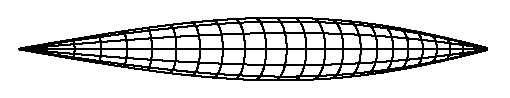
\includegraphics{asy/sin}
\vskip-0mm
\end{Figure}

Use \ref{ex:curvature-graph} and \ref{thm:meusnier} to show that the Gauss curvature of the surface of revolution of the graph $y=a\cdot \sin x$ for $x\in(0,\pi)$ cannot exceed $1$.
Try to support the surface $\Sigma$ from inside by a surface of revolution of the described type.
(Compare to \ref{ex:convex small}.)

\parit{Remark.}
The exercise can be deduced from the following deeper result: \textit{if the Gauss curvature of $\Sigma$ is at least $1$,
then
the intrinsic diameter of $\Sigma$ cannot exceed $\pi$}.
The latter means that any two points in $\Sigma$ can be connected by a path in $\Sigma$ that has length at most~$\pi$.
This theorem was proved by Heinz Hopf and Willi Rinow \cite{hopf-rinow} and 
named after Sumner Myers who generalized it \cite{myers}.

\parbf{\ref{ex:convex-proper-sphere}.}
To prove \ref{SHORT.ex:convex-proper-sphere:single} use the convexity of~$R$.
To prove \ref{SHORT.ex:convex-proper-sphere:smooth}, observe that the map $\Sigma\to\mathbb{S}^2$ is smooth and regular, then apply the inverse function theorem to show that its inverse is smooth as well.

\parbf{\ref{ex:convex-proper-plane}}; \ref{SHORT.ex:convex-proper-plane:a}
(The argument is similar to \ref{prop:convex-monotone:open}.)
We can assume that the origin lies on~$\Sigma$.
Consider a sequence of points $x_n\in \Sigma$ such that $|x_n|\z\to \infty$ as $n\to \infty$.
Denote by $\vec u_n$ the unit vector in the direction of $x_n$; that is $\vec u_n=\tfrac{x_n}{|x_n|}$.

Since the unit sphere is compact, we can pass to a subsequence of $(x_n)$ such that $\vec u_n$ converges to a unit vector, say $\vec u$.
Show that the half-line from the origin in the direction of $\vec u$ can be taken as $\ell$.


\parit{\ref{SHORT.ex:convex-proper-plane:b} $+$ \ref{SHORT.ex:convex-proper-plane:c} $+$ \ref{SHORT.ex:convex-proper-plane:d}.}
Since $R$ is convex, so is its projection $\Omega$.

Note and use that for any $q\in \Sigma$, the directions $\vec v_n=\tfrac{x_n-q}{|x_n-q|}$ converge to $\vec u$ as well.

\begin{wrapfigure}{r}{29 mm}
\vskip-0mm
\centering
\includegraphics{mppics/pic-1182}
\vskip-2mm
\end{wrapfigure}

Show that $\Sigma$ has no vertical tangent planes.
Conclude that the projection map from $\Sigma$ to the $(x,y)$-plane is regular.
Use the inverse function theorem to show that $\Omega$ is open.

\parit{\ref{SHORT.ex:convex-proper-plane:e}.} 
Arguing by contradiction, suppose for some sequence $(x_n,y_n)\z\to(x_\infty,y_\infty)\in \partial\Omega$ the sequence $f(x_n,y_n)$ stays bounded above.
We can pass to a subsequence such that either $f(x_n,y_n)$ converges to some finite value $z_\infty$ or it diverges to $-\infty$.

In the first case, show that the point $(x_\infty, y_\infty,z_\infty)$ does not lie on $\Sigma$, but it has arbitrarily close points on~$\Sigma$.
That is $\Sigma$ is not proper --- a contradiction.

If $f(x_n,y_n)\to -\infty$, use the convexity of $f$ to show that $f(\tfrac{x_n}2 ,\tfrac{y_n}2)\z\to -\infty$.
Note that the origin belongs to $\Omega$;
use it to show that $(\tfrac{x_\infty}2, \tfrac{y_\infty}2)\in\Omega$.
Arrive at a contradiction.

\parbf{\ref{ex:open+convex=plane}.}
By \ref{ex:convex-proper-plane:d}, $\Sigma$ is parametrized by an open convex plane domain $\Omega$.
It remains to show that $\Omega$ can parametrize the whole plane.

We may assume that the origin of the plane lies in $\Omega$.
Show that in this case, the boundary of $\Omega$ can be written in polar coordinates as $(\theta,f(\theta))$ where $f\:\mathbb{S}^1\to\mathbb{R}$ is a positive continuous function.
Then homeomorphism to the plane can be described in polar coordinates by changing only the radial coordinate;
for example, as 
$(\theta,r)\z\mapsto (\theta,
\tfrac{r}{1-r/f(\theta)})$.

To do the second part, one may apply \ref{ex:star-shaped-disc:nonsmooth}.


\parbf{\ref{ex:circular-cone}.}
Choose a coordinate system so that the $(x,y)$-plane supports $\Sigma$ at the origin, so $\Sigma$ lies in the upper half-space. 

Show that there is $\epsilon>0$ such that any line starting from the origin with slope at most $\epsilon$ may intersect $\Sigma$ only in the unit ball centered at the origin;
we may assume that $\epsilon$ is small, say $\epsilon<1$.
Consider the cone formed by the half-lines from the origin with slope $\epsilon$ shifted down by $1$.
Observe that the entire surface lies inside this cone.

\parbf{\ref{ex:intK}}.
Choose distinct points $p,q\in\Sigma$.
Apply \ref{thm:convex-embedded} to show that the angle 
$\measuredangle(\Norm(p),p-q)$ is acute and $\measuredangle(\Norm(q),p-q)$ is obtuse.
Conclude that $\Norm(p)\ne\Norm(q)$;
that is, $\Norm\:\Sigma\to\mathbb{S}^2$ is injective.

\parit{\ref{SHORT.ex:intK:4pi}.}
Given a unit vector $\vec u$, consider a point $p\in \Sigma$ that maximizes the scalar product $\langle p,\vec u\rangle$.
Show that $\Norm(p)=\vec u$.
Conclude that the spherical map $\Norm\:\Sigma\to\mathbb{S}^2$ is onto, and therefore it is a bijection.

Applying \ref{cor:intK}, we get that the integral is $4\cdot\pi=\area\mathbb{S}^2$.

\parit{\ref{SHORT.ex:intK:2pi}.} Choose an $(x,y,z)$-coordinate system provided by \ref{ex:convex-proper-plane:d}.
Observe that for any $p$ the normal vector $\Norm(p)$ forms an obtuse angle with the $z$-axis.
It follows that the image $\Norm(\Sigma)$ lies in the southern hemisphere.

Applying \ref{cor:intK}, we get that the integral is $2\cdot\pi=\tfrac12\cdot\area\mathbb{S}^2$.

\parbf{\ref{ex:convex-revolution}.}
Apply \ref{ex:principal-revolution}.

\parbf{\ref{ex:ruled=>saddle}.}
Prove and use that each point on the surface has a direction with vanishing normal curvature.

\parbf{\ref{ex:saddle-convex}.} Suppose $p\in \Sigma$ is a point of local maximum of~$f$.
Show that $\Sigma$ is supported by its tangent plane at~$p$.
Arrive at a contradiction.


\parbf{\ref{ex:panov}.}
Denote by $\Pi_t$ the affine tangent plane to $\Sigma$ at $\gamma(t)$ and by $\ell_t$ the tangent line to $\gamma$ at time~$t$.

Note that $\Pi_t$ is the graph of a linear function, say $h_t$, defined on the $(x, y)$-plane.
Denote by $\bar\ell_t$ the projection of $\ell_t$ to the $(x, y)$-plane.
Show that the derivative $\tfrac{d}{dt}h_t(w)$ vanishes at the point $w$ if and only if $w\in \bar\ell_t$ 
and the derivative changes sign if $w$ goes from one side of $\bar\ell_t$ to the other.

If $\bar\gamma$ is star-shaped with respect to a point $w$, then $w$ cannot cross $\bar\ell_t$.
Therefore, the function $t\mapsto h_t(w)$ is monotone on $\mathbb{S}^1$.
Observe that this function cannot be constant, and arrive at a contradiction.

\parbf{\ref{ex:crosss}.}
This problem follows easily from the so-called \index{Morse lemma}\emph{Morse lemma}.
The following sketch is a slightly stripped version of it.
A more conceptual proof \cite{palais} can be built on the Moser's trick; ses the solution of \ref{ex:star-shaped-disc}.

\medskip

Choose tangent-normal coordinates at $p$ so that the coordinate axes point in the principal directions of $\Sigma$ at $p$;
let $z=f(x,y)$ be the local graph representation of~$\Sigma$.
We need to show that the solution of the equation $f(x,y)=0$ is a union of two smooth curves that intersect transversely at~$p$.

Prove the following claim:
\begin{itemize}
\item Suppose $x\mapsto h(x)$ is a smooth function defined in an open interval $\mathbb{I}\ni0$ such that $h(0)=h'(0)=0$ and $h''(0)>0$.
Then, for a smaller interval $\mathbb{J}\ni0$ there is a unique smooth function $a\:\mathbb{J}\to\mathbb{R}$ such that $h=a^2$, $a(0)=0$ and $a'(0)> 0$.
\end{itemize}
Note that passing to a small rectangular domain $|x|,|y|<\epsilon$, we can assume that $f_{xx}>\epsilon$ and $f_{yy}<-\epsilon$. 
Show that if $\epsilon$ is small, then for every $x$ there is unique $y(x)$ such that $f_x(x,y(x))=0$; 
moreover, the function $x\mapsto y(x)$ is smooth.

Set $h(x)=f(x,y(x))$.
Note that $h(0)=h'(0)=0$ and $h''>0$.
Applying the claim, we get a function $a$ such that $h=a^2$, where $a(0)=0$ and $a'(0)>0$.

Observe that $g(x,y)=h(x)-f(x,y)\ge 0$, $g_y(x,y(x))\z=g(x,y(x))\z=0$, and $g_{yy}>0$.
Applying the claim to each function $y\mapsto g(x,y)$ with fixed $x$, we get that $g(x,y)=b(x,y)^2$ for a smooth function $b$ such that 
$b(x,y(x))=0$ and $b_y(x,y(x))>0$.

It follows that 
\begin{align*}
f(x,y)&=a(x)^2-b(x,y)^2=
\\
&=
(a(x)-b(x,y))\cdot (a(x)+b(x,y)).
\end{align*}
That is $f(x,y)=0$ if $a(x)\pm b(x,y) =0$.

It remains to observe that the two functions $g_\pm(x,y)=a(x)\pm b(x,y)$ have distinct non-zero gradients at $0$.
Therefore, each equation $a(x)\pm b(x,y) =0$ defines a smooth regular curve in a neighborhood of $p$;
see Section~\ref{sec:implicit-curves}.

\parbf{\ref{ex:length-of-bry}.}
Use \ref{lem:convex-saddle} and the hemisphere lemma (\ref{lem:hemisphere}).
For the second part, consider a thin cylindrical tube bounded by two closed spherical curves.

\parbf{\ref{ex:circular-cone-saddle}.}
Assume $\Sigma$ is an open saddle surface that lies in a cone~$K$.
Show that there is a plane $\Pi$ that cuts $\Sigma$ and cuts from $K$ a compact region.
Conclude that $\Pi$ cuts from $\Sigma$ a compact region as well. 

By \ref{lem:reg-section} one can move the plane $\Pi$ slightly so that it cuts from $\Sigma$ a compact surface with boundary.
Apply \ref{lem:convex-saddle}.


\parbf{\ref{ex:disc-hat}.} 
Consider the radial projection of $F_\epsilon$ to the sphere $\Sigma$ with center at $p=(0,0,\epsilon)$;
that is, a point $q\in F_\epsilon$ is mapped to a point $s(q)$ on the sphere that lies on the half-line $pq$.

Show that $s$ is a diffeomorphism from $F_\epsilon$ to the southern hemisphere of~$\Sigma$.
It remains to observe that the unit disc is diffeomorphic to the hemisphere.

\parbf{\ref{ex:saddle-linear}.} Apply \ref{prop:hat}.

\parbf{\ref{ex:between-parallels}.}
Find an example among the surfaces of revolution;
use \ref{ex:principal-revolution}.

\parbf{\ref{ex:one-side-bernshtein}.} Look at the sections of the graph by planes parallel to the $(x,y)$-plane and to the $(x,z)$-plane, then apply Meusnier’s theorem (\ref{thm:meusnier}).

\parbf{\ref{ex:saddle-graph}.}
Suppose the orthogonal projection of $\Sigma$ to the $(x,y)$-plane is not injective.
Show that there is a point $p\in\Sigma$ with a vertical tangent plane;
that is, $\T_p\Sigma$ is perpendicular to the $(x,y)$-plane.

Let $\Gamma_p$ be the connected component of $p$ in the intersection of $\Sigma$ and the affine tangent plane $\T_p\Sigma$.
Use \ref{ex:crosss} to show that $\Gamma_p$ is a union of smooth regular curves that can cross each other transversely.
Moreover, two of these curves pass thru $p$, and $\Gamma_p$ does not bound a compact region on~$\Sigma$.

Show that $\Gamma_p$ must have at least 4 ways to escape to infinity.
On the other hand, since $\Sigma$ is a graph outside the compact set $K$, we have that $\Gamma_p\backslash K$ is a graph of a real-to-real function that has only two ways to escape to infinity --- a contradiction.

\stepcounter{chapter}
\setcounter{eqtn}{0}

\begin{wrapfigure}{r}{24 mm}
\vskip-5mm
\centering
\includegraphics{mppics/pic-1250}
\vskip-0mm
\end{wrapfigure}

\parbf{\ref{ex:lasso}.}
Cut the lateral surface of the ice-mountain by a line from the cowboy to the tip.
Unfold it on the plane (see the picture) and try to figure out what is the image of the strained lasso.

\parbf{\ref{ex:length-dist-conv}.} 
Note that by \ref{thm:convex-embedded}, $\Sigma$ bounds a strictly convex region.
Therefore, we can assume that $\Norm(p)\ne\Norm(q)$; otherwise, $p=q$, and the inequality is evident.

Further, we can assume that $\Norm(p)+\Norm(q)\ne 0$; otherwise, the right-hand side is undefined.

In the remaining case, the tangent planes $\T_p$ and $\T_q$ intersect along a line, say $\ell$.
Set $\alpha=\tfrac12\cdot\measuredangle(\Norm(p),\Norm(q))$.
Show that $2\cdot\cos\alpha= |\Norm(p)+\Norm(q)|$.
Let $x\in \ell$ be the point that minimizes the sum $|p-x|\z+|x-q|$.
Show that $\measuredangle\hinge xpq\ge \pi-2\cdot\alpha$.
Conclude that 
\[|p-x|+|x-q|\le \frac{|p-q|}{\cos\alpha}.\]
Apply \ref{thm:shorts+convex} to show that
$\dist{p}{q}\Sigma\le |p-x|+|x-q|$.


\parbf{\ref{ex:hat-convex}.}
Suppose there is a minimizing curve $\gamma\not\subset\Delta$ with endpoints $p$ and $q$ in $\Delta$.

Without loss of generality, we may assume that only one arc of $\gamma$ lies outside $\Delta$.
Reflection of this arc with respect to $\Pi$ together with the remaining part of $\gamma$ forms another curve $\hat\gamma$ from $p$ to $q$;
it runs partly along $\Sigma$ 
and partly outside $\Sigma$,
but does not get inside.
Note that
\[\length\hat\gamma=\length\gamma.\]


Denote by $\bar\gamma$ the closest-point projection of $\hat\gamma$ on~$\Sigma$.
The curve $\bar\gamma$ lies in $\Sigma$, 
it has the same endpoints as $\gamma$,
and by \ref{thm:shorts+convex}
\[\length\bar\gamma<\length\gamma.\]
This means that $\gamma$ is not length minimizing --- 
a contradiction.

\parbf{\ref{ex:intrinsic-diameter}.} 
Show that the closest-point projection $\partial B\to\Sigma$ is surjective, and apply \ref{lem:closest-point-projection}.

\stepcounter{chapter}
\setcounter{eqtn}{0}


\parbf{\ref{ex:clairaut}.} 
We can assume that the origin lies on the axis of revolution, and $\vec i$ points in the direction of such axis.
Use \ref{lem:constant-speed} to show that it is sufficient to prove that 
$\langle\gamma'\times \gamma,\vec i\rangle$
is constant.

Since $\gamma''(t)\perp\T_{\gamma(t)}$, the three vectors $\vec i$, $\gamma$, and $\gamma''$ lie in the same plane.
In particular, $\langle\gamma''\times \gamma,\vec i\rangle=0$.
Therefore,
$
\langle\gamma'\times \gamma,\vec i\rangle'
=
\langle\gamma'\times \gamma',\vec i\rangle+\langle\gamma''\times \gamma,\vec i\rangle =0
$.



\parbf{\ref{ex:asymptotic-geodesic}.} By Lemma \ref{lem:constant-speed},
we can assume that $\gamma$ is parametrized by arc-length.
By the definition of geodesic, we have that $\gamma''(s)\perp\T_{\gamma(s)}$. 
Therefore, 
\[\gamma''(s)=k_n(s)\cdot\Norm(\gamma(s)),\]
where $k_n(s)$ is the normal curvature of $\gamma$ at time~$s$.
Since $\gamma$ is asymptotic, $k_n(s)\equiv 0$;
that is, $\gamma''(s)\equiv 0$, therefore $\gamma'$ is constant and hence $\gamma$ runs along a line segment; see \ref{ex:zero-curvature-curve}.




\parbf{\ref{ex:reflection-geodesic}.}
Denote by $\mu$ a unit vector perpendicular to $\Pi$.
Since $\gamma$ lies in $\Pi$, we have that $\gamma''$ is parallel to $\Pi$, or equivalently $\gamma''\perp \mu$.
Since $\gamma$ is unit speed, \ref{prop:a'-pertp-a''} implies that $\gamma''\perp\gamma'$.

Since $\Sigma$ is mirror-symmetric with respect to the plane $\Pi$,
the tangent plane $\T_{\gamma(t)}\Sigma$ is also mirror-symmetric with respect to $\Pi$.
It follows that $\T_{\gamma(t)}\Sigma$ is spanned by $\mu$ and $\gamma'(t)$.
Hence, $\gamma''\perp \mu$ and $\gamma''\perp\gamma'$ imply $\gamma''\perp\T_{\gamma(t)}\Sigma$;
that is, $\gamma$ is a geodesic.



\parbf{\ref{ex:round-torus}.}
By \ref{ex:reflection-geodesic}, any meridian of $\Sigma$ is a closed geodesic.
Consider an arbitrary closed geodesic~$\gamma$.

If $\gamma$ is tangent to a meridian at some point, then by the uniqueness part of Proposition \ref{prop:geod-existence}, $\gamma$ runs along that meridian;
in particular, it is non-contractible.

In the remaining case, $\gamma$ can intersect meridians only transversely.
Therefore, the longitude of $\gamma$ is monotone.
Whence again $\gamma$ is non-contractible.


\parbf{\ref{ex:helix=geodesic}.}
Show that $\Norm(\gamma(t))=(\cos t,\sin t, 0)$.
Calculate $\gamma''(t)$, and show that it is proportional to $\Norm(\gamma(t))$.
The latter is equivalent to $\gamma''(t)\perp\T_{\gamma(t)}$. 
Note that the line segment from $\gamma (0) $ to $\gamma (2 \pi) $ is contained in~$\Sigma$.



\parbf{\ref{ex:two-min-geod}.}
Assume two shortest paths $\alpha$ and $\beta$ have two common points $p$ and~$q$.
Denote by $\alpha_1$ and $\beta_1$ the arcs of $\alpha$ and $\beta$ from $p$ to~$q$.
Suppose $\alpha_1$ is distinct from $\beta_1$.

Note that $\alpha_1$ and $\beta_1$ are shortest paths with the same endpoints;
in particular, they have the same length.
Exchanging $\alpha_1$ in $\alpha$ to $\beta_1$ produces a shortest path, say $\hat\alpha$, that is distinct from $\alpha$.
By \ref{prop:gamma''}, $\hat\alpha$ is a geodesic.

Suppose $\alpha_1$ is a proper subarc of $\alpha$;
that is, $\alpha_1\ne\alpha$, or equivalently, either $p$ or $q$ is not an endpoint of $\alpha$.
Then $\alpha$ and $\hat\alpha$ share one point and velocity vector at this point.
By \ref{prop:geod-existence} $\alpha$ coincides with $\hat\alpha$ --- a contradiction.

{

\begin{wrapfigure}{r}{38 mm}
\vskip-4mm
\centering
\includegraphics{mppics/pic-308}
\vskip0mm
\end{wrapfigure}

It follows that $p$ and $q$ are the endpoints of $\alpha$.
Analogously, $p$ and $q$ are the endpoints of $\beta$.


For the second part, one could consider two distinct curves of the form 
\[ \gamma_b(t) = ( \cos t , \sin t , bt ) , t \in \mathbb{R} \]
in the cylinder $x^2 + y^2 =1$.

}

\parbf{\ref{ex:min-geod+plane}.}
Assume a shortest path $\alpha$ crosses $\Pi$ at least twice.
In this case, there is an subarc $\alpha_1$ of $\alpha$ that lies entirely on one side
 on $\Pi$, has endpoints on $\Pi$, and these endpoints are distinct from the endpoints of $\alpha$.
 
\begin{wrapfigure}{r}{38 mm}
\vskip-6mm
\centering
\includegraphics{mppics/pic-310}
\vskip0mm
\end{wrapfigure}

Let us remove the arc $\alpha_1$ from $\alpha$ and replace it with the reflection of $\alpha_1$ across $\Pi$.
Note that the obtained curve, say $\beta$, lies in the surface;
it has the same length as $\alpha$, and it connects the same pair of points, say $p$ and~$q$.
Therefore, $\beta$ is another shortest path from $p$ to $q$ in $\Sigma$ that is distinct from~$\alpha$.

We may assume that both $\alpha$ and $\beta$ have arc-length parametrization.
By \ref{prop:gamma''}, $\alpha$ and $\beta$ are geodesics.
Since $\alpha$ and $\beta$ have a common subarc, they share one point and velocity vector at this point;
by \ref{prop:geod-existence} $\alpha$ coincides with $\beta$ --- a contradiction.

\parbf{\ref{ex:milka}.} Let $W$ be the closed region outside~$\Sigma$.
Show that the distance $\dist{p^t}{q}W$ is constant with respect to~$t$.
This implies that the concatenation of the line segment $[p^t,\gamma(t)]$ and the arc $\gamma|_{[t,\ell]}$ is a shortest path from $p^t$ to $q$ in~$W$.

Since $\Sigma$ is strictly convex, 
\[ \dist{\gamma (t)}{q}W > \dist{\gamma(t)}{q}{\mathbb{R}^3} \]
for all $t < \ell$.
Hence,
\begin{align*}
\dist{p^t}{q}W&=\dist{p^t}{\gamma(t)}W+\dist{\gamma (t)}{q}W 
> 
\\
&>\dist{p^t}{\gamma(t)}{\mathbb{R}^3} + \dist{ \gamma (t)}{q}{\mathbb{R}^3} 
\ge
\\
&\ge\dist{p^t}{q}{\mathbb{R}^3}. 
\end{align*}
If the segment $[p^t , q ]$ was entirely contained in $W$ for some $t< \ell $, then $ \dist{p^t}{q}W = \dist{p^t}{q}{\mathbb{R}^3} $, which would be a contradiction.

\parbf{\ref{ex:rho''}.}
Equip $\Sigma$ with unit normal field $\Norm$ that points inside.
Denote by $k(t)$ the normal curvature of $\Sigma$ at $\gamma(t)$ in the direction of $\gamma'(t)$.
Since $\Sigma$ is convex, $k(t)\ge 0$ for any~$t$.

Since $\gamma$ is a unit-speed geodesic, we have $\gamma''(t)=k(t)\cdot\Norm(\gamma(t))$ and $\langle\gamma'(t),\gamma'(t)\rangle=1$ for any~$t$.
Without loss of generality, we can assume that $p$ is the origin of~$\mathbb{R}^3$.
Since $p$ is inside $\Sigma$, we have that $\langle\gamma(t),\Norm(\gamma(t))\rangle\le 0$ for any~$t$.
It follows that 
\[\langle\gamma''(t),\gamma(t)\rangle=k(t)\cdot \langle\gamma(t),\Norm(\gamma(t))\rangle\le 0\]
for any~$t$.

Applying the above estimates, we get 
\begin{align*}
\rho''(t)
&=\langle\gamma(t),\gamma(t)\rangle''=
\\
&=2\cdot\langle\gamma''(t),\gamma(t)\rangle+2\cdot\langle\gamma'(t),\gamma'(t)\rangle\le
\\
&\le 2.
\end{align*}


\parbf{\ref{ex:tc-spherical-image}.}
We can assume $\gamma$ is unit-speed.
Set $\nu (t) = \nu ( \gamma (t)) $. 
Then $\langle \gamma'(t) , \nu (t) \rangle \equiv 0$. Also, since $\gamma$ is a geodesic, we have that $\gamma''(t) \parallel \nu (t)$.
Therefore,
\[
\begin{aligned}
|\gamma''(t)|
&=|\langle\gamma''(t),\nu(t)\rangle|=
\\
&=|\langle\gamma'(t),\nu(t)\rangle'-\langle\gamma'(t),\nu'(t)\rangle|=
\\
&=|\langle\gamma'(t),\nu'(t)\rangle|\le
\\
&\le|\gamma'(t)||\nu'(t)|=|\nu'(t)|.
\end{aligned}
\]

Integrating both sides with respect to $t$, we get 
\[\length(\Norm\circ\gamma)\ge \tc\gamma.\]

\parbf{\ref{ex:usov-exact}.} 
Suppose $\gamma(t)=(x(t),y(t),z(t))$. 
Show that
\[|\gamma'' (t)| = z''(t)\cdot\sqrt{1+ \ell ^2}\eqlbl{eq:gamma''=z''}\]
for any~$t$.

Observe that $z'(t)\to\pm \tfrac\ell{\sqrt{1+ \ell ^2}}$ as $t\to\pm\infty$.
Conclude that 
\[\int_{-\infty}^{+\infty}z''(t)\cdot dt
=
\frac{2\cdot\ell}{\sqrt{1+ \ell ^2}}.\eqlbl{eq:int z''}\]
By \ref{eq:gamma''=z''} and \ref{eq:int z''}, we have
\begin{align*}
\tc\gamma&=\int_{-\infty}^{+\infty}|\gamma''(t)|\cdot dt=
\\
&=
\sqrt{1+ \ell ^2}\cdot \int_{-\infty}^{+\infty}z''(t)\cdot dt=
\\
&=2\cdot \ell.
\end{align*}

\parbf{\ref{ex:ruf-bound-mountain}.}
Use \ref{thm:usov} and \ref{ex:sef-intersection}.
For the second part, consider a geodesic on a cone with slope $2$, and mollify its tip.

\parit{Remark.}
The statement still holds for $\sqrt{3}$-Lipschitz functions, and $\sqrt{3}=\tg\tfrac\pi3$ is the optimal bound; see \ref{ex:sqrt(3)}.
It is the same slope as in the problem about the cowboy and the lasso (\ref{ex:lasso}).

\parbf{\ref{ex:parallel}}; \ref{SHORT.ex:parallel:a}.
Show and use that $\langle\vec v(t),\vec v'(t)\rangle=0$.

\parit{\ref{SHORT.ex:parallel:b}}
Show that $|\vec v(t)|$, $|\vec w(t)|$, and
$\langle\vec v(t),\vec w(t)\rangle=0$,
are constants; it can be done the same way as \ref{SHORT.ex:parallel:a}.
Then use that 
$\langle\vec v(t),\vec w(t)\rangle=|\vec v(t)|\cdot|\vec w(t)|\cdot\cos\theta$.

\stepcounter{chapter}
\setcounter{eqtn}{0}

\parbf{\ref{ex:parallel-transport-support}.}
Observe that $\Sigma_1$ supports $\Sigma_2$ at any point of~$\gamma$.
Conclude that $\gamma$ has identical spherical images as a curve in $\Sigma_1$ and in $\Sigma_2$.
Apply \ref{obs:parallel=}.

\parbf{\ref{ex:holonomy=not0}.}
Nearly any loop solves the problem.
For example, consider the right-angled spherical triangle that an octant of $\mathbb{R}^3$ cuts form the sphere.
Argue that parallel transport around it rotates the tangent plane by the angle $\tfrac\pi 2$. 

\stepcounter{chapter}
\setcounter{eqtn}{0}

\parbf{\ref{ex:1=geodesic-curvature}.}
By \ref{ex:convex-proper-sphere}, $\Sigma$ is a smooth sphere.
By Jordan theorem (\ref{thm:jordan}) the curve $\gamma$ divides $\Sigma$ into two discs.
Let us denote by $\Delta$ the disc that lies on the left from~$\gamma$.

Observe that $\tgc\gamma=\length\gamma$, and apply the Gauss--Bonnet formula (\ref{thm:gb}) for $\Delta$.

\parbf{\ref{ex:geodesic-half}.}
Apply \ref{cor:intK}, \ref{ex:intK:4pi}, and the Gauss--Bonnet formula (\ref{thm:gb}).
For the last part, apply \ref{ex:bisection-of-S2}.

\parbf{\ref{ex:closed-geodesic}.} For the first part apply the Gauss--Bonnet formula (\ref{thm:gb}).

For the second part, arguing by contradiction, assume two closed geodesics $\gamma_1$ and $\gamma_2$ do not intersect. 
This would imply that $\gamma_2$ lies in one of the regions, say $R_1$, that $\gamma_1$ cuts from~$\Sigma$.
Similarly, $\gamma_1$ lies in one of the regions, say $R_2$, that $\gamma_2$ cuts from~$\Sigma$.

Observe that $R_1$ and $R_2$ cover $\Sigma$ with overlap.
Therefore, the first part implies that the integral of the Gauss curvature over $\Sigma$ is less than $4\cdot\pi$.
The latter contradicts \ref{ex:intK:4pi}.

\parbf{\ref{ex:self-intersections}}; \textit{(easy)}.
Consider the 4 regions bounded by loops.
Apply the Gauss--Bonnet formula (\ref{thm:gb}) to show that the integral of the Gauss curvature on each of these regions exceeds $\pi$.
The latter contradicts \ref{ex:intK:4pi}.

\parit{(tricky)}.
Denote by $\alpha$, $\beta$, and $\gamma$ the angles of the triangle.
Apply the Gauss--Bonnet formula (\ref{thm:gb}) to show that the loops surround regions over which the integral of the Gauss curvature is $\pi+\alpha$, $\pi+\beta$, and $\pi+\gamma$, respectively.

Apply the Gauss--Bonnet formula to the triangular region to show that $\alpha+\beta+\gamma>\pi$.
Use \ref{ex:intK:4pi} to get at a contradiction.

\parbf{\ref{ex:sqrt(3)}.} Note that it is sufficient to show that the surface has no geodesic loops.
Estimate the integrals of the Gauss curvature over the entire surface and a disc surrounded by a geodesic loop.

\parbf{\ref{ex:unique-geod}}; \ref{SHORT.ex:unique-geod:unique}.
By \ref{prop:shortest-paths-exist} and \ref{prop:gamma''}, any two points in $\Sigma$ can be connected by a geodesic.
Suppose points $p$ and $q$ can be connected by two distinct geodesics $\gamma_1$ and $\gamma_2$.
Passing to their subarcs, we may assume that $\gamma_1$ and $\gamma_2$ share only their endpoints.
Since the surface is simply-connected, $\gamma_1$ and $\gamma_2$ together bound a disc, say $\Delta\subset\Sigma$.
It remains to apply the Gauss--Bonnet formula to $\Delta$ and make a conclusion.
 
\parit{\ref{SHORT.ex:unique-geod:diffeomorphism}.} 
Use part \ref{SHORT.ex:unique-geod:unique} and \ref{prop:inj-rad}.

\parbf{\ref{ex:half-sphere-total-curvature}.}
Apply \ref{prop:pt+tgc} and \ref{prop:area-of-spher-polygon}.

\parbf{\ref{ex:cohn-vossen}.}
Repeat the end of the proof of \ref{thm:cohn-vossen} for a one-parameter family of geodesics $\gamma_\tau$ defined by $\gamma_\tau(0)=\alpha(\tau)$ and $\gamma'(0)=\alpha'(\tau)$. 

\stepcounter{chapter}
\setcounter{eqtn}{0}

\parbf{\ref{ex:semigeodesc-chart}.}
By the Gauss lemma (\ref{lem:palar-perp}), polar coordinates with respect to $q$ produce a semigeodesic chart at any nearby point.
Therefore, it is sufficient to find a point $q\ne p$ such that polar coordinates on $\Sigma$ with respect to $q$ cover~$p$.
By \ref{prop:exp}, any $q$ sufficiently close to $p$ does the job.

\parbf{\ref{ex:inj-rad}}; \ref{SHORT.ex:inj-rad:sign}.
Show that we can choose an orientation on $\Sigma$ so that $b_r(0,\theta)\z=1$ for any $\theta$.
Conclude that we can assume that $b(r,\theta)>0$ for all small $r>0$.

Suppose $b(r_1,\theta_1)<0$ at some pair $(r_1,\theta_1)$ with $0<r_1<r_0$.
Observe that if $\theta_2$ is sufficiency close to $\theta_1$, then the radial curves $r\mapsto b(r,\theta_1)$ and $r\mapsto b(r,\theta_2)$ defined on the interval $(0,r_1)$ intersect.
Therefore, $\exp_p$ is not injective in $B$ --- a contradiction.

\parit{\ref{SHORT.ex:inj-rad:0}.}
Suppose $b(r_1,\theta_1)=0$.
Apply \ref{SHORT.ex:inj-rad:sign} to show that $b_r(r_1,\theta_1)=0$.

Apply \ref{prop:jaccobi} to conclude $b(r,\theta_1)=0$ for any~$r$.
The latter contradicts that $b_r(0,\theta_1)=1$.

\parit{\ref{SHORT.ex:inj-rad:prop:inj-rad}.}
We need to show that $\exp_p$ is regular in~$B$.
Suppose vector $\vec v\in B$ has polar coordinates $(r,\theta)$ for some $r>0$.
Show that $\exp_p$ is regular at $\vec v$ if $b(r,\theta)\ne 0$.
Conclude that $\exp_p$ is regular in $B\backslash \{0\}$.

By \ref{obs:d(exp)=1}, $\exp_p$ is regular at $0$.
Whence $\exp_p|_B$ is a regular injective smooth map.
Use the inverse function theorem (\ref{thm:inverse}) to show that the restriction $\exp_p|_B$ is a diffeomorphism to its image. 
 



\parbf{\ref{lem:K(orthogonal)}}; \ref{SHORT.lem:K(orthogonal):uu-vv}.
Since the frame $\vec u, \vec v,\Norm$ is orthonormal,
the first two vector identities are equivalent to the following six real identities:
\[
\begin{aligned}
\langle\vec u_u,\vec u\rangle
&=0,
&
\langle\vec u_u,\vec v\rangle
&=-\tfrac1{b}\cdot a_v,
&
\langle\vec u_u,\Norm\rangle
&=a\cdot \ell,
\\
\langle\vec v_u,\vec v\rangle
&=0,
&
\langle\vec v_u,\vec u\rangle
&=
\tfrac1{b}\cdot a_v,
&
\langle\vec v_u,\Norm\rangle
&=
a\cdot m.
\end{aligned}
\eqlbl{eq:key-orthogonal/2}
\]

Taking the partial derivatives of the identities
$\langle\vec u,\vec u\rangle=1$ and
$\langle\vec v,\vec v\rangle=1$ with respect to $u$,
we get the first two identities in \ref{eq:key-orthogonal/2}.

Further, observe that
\[
\begin{aligned}
\vec v_u
&=
\tfrac{\partial}{\partial v}
(\tfrac1b\cdot s_v)=\tfrac1b\cdot s_{uv}
+
\tfrac{\partial}{\partial u}(\tfrac1b)
\cdot
 s_v.
\end{aligned}
\eqlbl{eq:dv/du}
\]
Since $s_u\perp s_v$, it follows that
\begin{align*}
\langle\vec v_u,\vec u\rangle
&=
\tfrac1{a\cdot b}\cdot \langle s_{vu}, s_u\rangle=
\\
&=
\tfrac1{2\cdot a\cdot b}\cdot \tfrac{\partial}{\partial v}\langle s_u, s_u\rangle=
\tfrac1{2\cdot a\cdot b}\cdot \tfrac{\partial a^2}{\partial v}=
\\
&=
\tfrac1{b}\cdot a_v.
\end{align*}
Taking the partial derivative of $\langle\vec u,\vec v\rangle=0$ with respect to $u$
we get
\begin{align*}
\langle\vec v_u,\vec u\rangle+
\langle\vec v,\vec u_u\rangle
&=0.
\end{align*}
Hence, we get two more identities in \ref{eq:key-orthogonal/2}.

Since $\vec u, \vec v$ is an orthonormal frame, by \ref{thm:shape-chart} we have
\[
\begin{aligned}
\tfrac1{a^2}
\cdot
\langle s_{uu},\Norm\rangle
&=\ell,
&
\tfrac1{a\cdot b}
\cdot
\langle s_{uv},\Norm\rangle
&=m,
\\
\tfrac1{a\cdot b}
\cdot
\langle s_{vu},\Norm\rangle
&=m,
&
\tfrac1{b^2}
\cdot
\langle s_{vv},\Norm\rangle
&=n.
\end{aligned}
\eqlbl{eq:shape-lmn}
\]

Applying \ref{eq:dv/du}, \ref{eq:shape-lmn}, and $s_v\perp\Norm$ we get
\begin{align*}
\langle\vec u_u,\Norm\rangle
&=
\tfrac1{a}\cdot \langle s_{uu},\Norm\rangle
=a\cdot \ell,
\\
\langle\vec v_u,\Norm\rangle
&=
\tfrac1{a}\cdot \langle s_{uv},\Norm\rangle
=a\cdot m,
\end{align*}
that imply the last two equalities in \ref{eq:key-orthogonal/2}.

Therefore, the first two identities in \ref{SHORT.lem:K(orthogonal):uu-vv} are proved;
the remaining two identities can be proved along the same lines.

\parit{\ref{SHORT.lem:K(orthogonal):K}.}
Recall that the Gauss curvature equals the determinant of the matrix $
(\begin{smallmatrix}
\ell&m
\\
m&n
\end{smallmatrix}
)
$;
that is, $K=\ell\cdot n-m^2$.
Therefore, 
\begin{align*}
a\cdot b\cdot K
&=
a\cdot b\cdot(\ell\cdot n-m^2)
=
\\
&=
\langle\vec u_u,\vec v_v\rangle 
-
\langle\vec u_v,\vec v_u\rangle= 
\\
&= 
\left(
\tfrac{\partial}{\partial v}
\langle\vec u_u,\vec v\rangle
-
\cancel{\langle\vec u_{uv},\vec v\rangle}
\right)-
\\
&-
\left(
\tfrac{\partial}{\partial u}
\langle\vec u_v,\vec v\rangle
-
\cancel{\langle\vec u_{uv},\vec v\rangle}
\right)=
\\
&=\tfrac{\partial}{\partial v}(-\tfrac1{b}\cdot a_v)
-
\tfrac{\partial}{\partial u}(\tfrac1{a}\cdot b_u).
\end{align*}

\parbf{\ref{ex:conformal}.}
Apply \ref{lem:K(orthogonal)} assuming that $a=b$, and simplify.

\parbf{\ref{ex:K=0}.}
Note and use that by \ref{prop:rauch}, $\exp_p$ is length-preserving.

\parbf{\ref{ex:K=1}.} Modify the proof of \ref{prop:rauch} to show that $K\equiv 1$ implies that $b(\theta,r)\z=\sin r$ for all small $r\ge 0$.



\parbf{\ref{ex:deformation}.}
To find $x(t)$, one may solve the differential equation
$x'(t)=\sqrt{1-|y'(t)|^2}$.
Its solution is defined on any interval where $|y'(t)|=|a\cdot \sin t|<1$ holds.

Apply \ref{ex:principal-revolution:formula} to calculate Gauss curvature of $\Sigma_a$.

By \ref{ex:K=1}, small discs $\Delta_a$ in $\Sigma_a$ admit intrinsic isometry to a disc in a unit sphere.
To show that $\Delta_a$ is not congruent to a spherical disc $\Delta_1$ for $a\ne 1$, show that its principle curvature is not 1 at some point. 

\stepcounter{chapter}
\setcounter{eqtn}{0}

\parbf{\ref{ex:wide-hinges}.}
Apply the triangle inequality $c_n\le a_n+b_n$ and the bound $a_n,b_n>\epsilon$ to show that the sequence 
\[\frac{a_n+b_n+c_n}{2\cdot a_n\cdot b_n}\]
is bounded.
Conclude that 
\[\frac{(a_n+b_n)^2-c_n^2}{2\cdot a_n\cdot b_n}=\frac{(a_n+b_n+c_n)\cdot(a_n+b_n-c_n)}{2\cdot a_n\cdot b_n}\to 0\]
as $n\to\infty$.

Use the last statement together with the cosine rule
\[a_n^2+b_n^2-2\cdot a_n\cdot b_n\cdot\cos\tilde\theta_n -c_n^2=0\]
to show that $\cos\tilde\theta_n\to -1$ as $n\to\infty$;
conclude that $\theta_n\to \pi$.

\parbf{\ref{ex:thm:comp:cat:nsc}.}
Consider the triangle on the hyperboloid with vertices $(1,0,0)$, $(-\tfrac{1}2, \tfrac{\sqrt{3} }2, 0)$, and $(-\tfrac{1}2, -\tfrac{\sqrt{3} }2, 0)$.
Note that all its angles equal to $\pi$, but all model angles equal to $\tfrac{\pi}3$.

\parbf{\ref{ex:diam-angle}.}
Show that $\dist{p}{x}\Sigma\le \dist{p}{q}\Sigma$ and $\dist{q}{x}\Sigma\le \dist{p}{q}\Sigma$.
Conclude that $\modangle xpq\ge \tfrac\pi3$.
Apply \ref{thm:comp:toponogov}.

\parbf{\ref{ex:sum=<2pi}.}
Show that 
$\measuredangle\hinge pxy+\measuredangle\hinge pyz+\measuredangle\hinge pzx\le2\cdot \pi$.
Apply \ref{thm:comp:toponogov}.

\parbf{\ref{ex:s-r}.}
Choose vectors $\vec u$, and $\vec w$ 
such that $|\vec w|=\dist{p}{x}{}$, $|\vec u|=1$, and $\measuredangle(\vec u,\vec w)=\measuredangle\hinge xpq$.
Consider the function
$f\:t\mapsto t+|\vec w|-|\vec w-t\cdot \vec u|$.
Set $t_0=\dist{x}{y}{}$ and $t_1=\dist{x}{q}{}$.
Observe that 
\begin{align*}
f(t_0)&=\dist{x}{p}{}+\dist{x}{y}{}-\side\hinge xpy,
\\
f(t_1)&=\dist{x}{p}{}+\dist{x}{q}{}-\side\hinge xpq.
\end{align*}

Show and use that $f$ is concave and $f(0)=0$.

\parbf{\ref{ex:open-comparison}}; \ref{SHORT.ex:open-comparison:positive}.
Apply Rauch comparison \ref{prop:rauch} and properties of the exponential map in \ref{prop:exp}.

\parit{\ref{SHORT.ex:open-comparison:almost-min}.} Argue by contradiction.
If the statement does not hold, then for any $p\in\Sigma$ there is a point $q=q(p)\in \Sigma$ such that 
$\dist{q}{p}\Sigma< 100\cdot R_p$
and
$R_q<(1-\tfrac1{100})\cdot R_p$.

Start with any point $p_0$, and consider a sequence $p_n$ defined by $p_{n+1}\z\df q(p_n)$.
Show that $p_n$ converges, and $R_{p_n}\to 0$ as $n\to\infty$.
Arrive at a contradiction using \ref{SHORT.ex:open-comparison:positive}.

\parit{\ref{SHORT.ex:open-comparison:proof}.} Repeat the proof assuming that $p$ is provided by \ref{SHORT.ex:open-comparison:almost-min}.

\parbf{\ref{ex:convex-polyhon+self-intersections}.}
A complete solution is given in \cite{petrunin2021}.

\parit{\ref{SHORT.ex:convex-polyhon+self-intersections:angles}.}
Apply the Gauss--Bonnet formula for each region that $\gamma$ cuts from $\Sigma$, and simplify the obtained inequalities.

\begin{Figure}
\vskip-0mm
\centering
\includegraphics{mppics/pic-474}
\vskip-0mm
\end{Figure}

\parit{\ref{SHORT.ex:convex-polyhon}.}
Consider the pentagon $\Delta$ with induced length-metric.
Note that all its angles cannot exceed $\pi$.
Repeat the proof of \ref{thm:comp:toponogov} to show that the comparison holds in $\Delta$.

Choose a vertex $v$ of $\Delta$. 
Subdivide the sides of $\Delta$ so that each arc of the subdivision is a minimizing geodesic, so the boundary of $\Delta$ is a broken geodesic.
Divide $\Delta$ into triangles by joining $v$ to other vertices of the broken geodesic.
Take a model triangle for each so that they shared sides as in $\Delta$.
Use the comparison to show that these plane triangles form a required polygon.

\parit{\ref{SHORT.ex:self-intersections-hard}}.
It remains to show that the plane pentagon provided by \ref{SHORT.ex:convex-polyhon} cannot exist.
Imagine that there is some air pressure in the pentagon, it should not move it; so the net force should vanish.
Use part \ref{SHORT.ex:convex-polyhon+self-intersections:angles} to show that this is not the case.
(Equivalently, show that the sum of its side vectors oriented counterclockwise does not vanish.)

\parbf{\ref{ex:geod-convexity}.}
Apply \ref{angk>angk} and \ref{angk<angk}.

\parbf{\ref{ex:midpoints}.} Use \ref{angk>angk} or \ref{angk<angk} twice:
first --- for the triangle $[pxy]$ and $\bar x\in [p,x]$;
second --- for the triangle $[p\bar xy]$ and $\bar y\in [p,y]$.
Then apply the angle monotonicity (\ref{lem:angle-monotonicity}).

\parbf{\ref{ex:convex-dist}.}
It is sufficient to prove the Jensen inequality;
that is, 
\[
\dist{\gamma_1(\tfrac12)}{\gamma_2(\tfrac12)}{}
\le
\tfrac12\cdot\dist{\gamma_1(0)}{\gamma_2(0)}{}
+
\tfrac12\cdot \dist{\gamma_1(1)}{\gamma_2(1)}{}.
\]

\begin{Figure}
\vskip-0mm
\centering
\includegraphics{mppics/pic-1650}
\end{Figure}

Let $\delta$ be the geodesic path from $\gamma_2(0)$ to $\gamma_1(1)$.
From \ref{ex:midpoints}, we have
\begin{align*}
\dist{\gamma_1(\tfrac12)}{\delta(\tfrac12)}{}
&\le
\tfrac12\cdot\dist{\gamma_1(0)}{\delta(0)}{},
\\
\dist{\delta(\tfrac12)}{\gamma_2(\tfrac12)}{}
&\le
\tfrac12\cdot\dist{\delta(1)}{\gamma_2(1)}{},
\end{align*}
Sum it up, and apply the triangle inequality.

\parit{Remark.} Note that modulo the comparison theorem, 
the case of the Euclidean plane is just as hard.

\parbf{\ref{ex:dist-to-bry}}; \ref{SHORT.ex:dist-to-bry:-}.
Choose two points $x,z\in\Sigma$;
let $y$ be the midpoint of $[x,z]$.
Denote by $\bar x$ and $\bar z$ the points on $\delta$ that minimize the distances to $x$ and $z$, respectively;
so we have
$f(x)
=\dist{x}{\bar x}\Sigma$,
and $f(z)=\dist{z}{\bar z}\Sigma$.

Since $\Delta$ is convex, the midpoint of $[\bar x,\bar z]$, say $\bar y$, lies in $\Delta$.
By \ref{ex:convex-dist}, we have 
\begin{align*}
f(y)&\le \dist{y}{\bar y}\Sigma
\le
\\
&\le
\tfrac12\cdot(\dist{x}{\bar x}\Sigma
+
\dist{z}{\bar z}\Sigma)
=
\\
&=
\tfrac12\cdot(f(x)+f(z)).
\end{align*}
Observe that this inequality implies the convexity of ~$f$.

\parit{\ref{SHORT.ex:dist-to-bry:+}.}
Suppose $\gamma$ is a unit-speed geodesic in $\Delta$, and $\gamma(0)=p$. 
Let $q$ be a point on $\delta$ that minimize the distance to~$p$.
Denote by $\phi$ the angle between $\gamma$ and $[p,q]$ at~$p$.
Note that it is sufficient to show that 
\[f\circ\gamma(t)\le 
\dist{p}{q}\Sigma+t\cdot\cos\phi\eqlbl{eq:dist<cosphi}\]
for $t$ sufficiently close to~$0$.

\begin{Figure}
\vskip-0mm
\centering
\includegraphics{mppics/pic-1680}
\vskip0mm
\end{Figure}

Chose small $t>0$, and set $x\z=\gamma(t)$.
Consider a model triangle $[\tilde p\tilde q\tilde x]\z=\tilde\triangle(pqx)$.
Let $\tilde\delta$ be the line thru $\tilde q$ perpendicular to $[\tilde p,\tilde q]$.
Denote by $\tilde y$ the orthogonal projection of $\tilde x$ to $\tilde\delta$.
By comparison, we have that 
\begin{align*}
\phi
=\measuredangle\hinge qpx
&\ge \modangle qpx
\mathrel{=:}\tilde\phi,
\\
\psi\df
\measuredangle\hinge pqx
&\ge 
\modangle pqx
\mathrel{=:}\tilde \psi
\end{align*}

Since $t=\dist{\tilde p}{\tilde x}{\mathbb{R}^2}$ is small, so is the distances $\dist{\tilde q}{\tilde y}{\mathbb{R}^2}$.
Therefore, we can choose a point $y$ on $\delta$ such that $\dist{q}{y}\Sigma=\dist{\tilde q}{\tilde y}{\mathbb{R}^2}$.
Moreover, if we choose in on the {}\emph{right side}, then $\tfrac\pi2-\psi \ge \measuredangle\hinge qxy$.
By construction and comparison, we have 
\begin{align*}
\measuredangle\hinge {\tilde q}{\tilde x}{\tilde y}&=\tfrac\pi2-\tilde\psi
\ge
\tfrac\pi2-\psi
\ge
\measuredangle\hinge q x y
\ge 
\modangle q x y.
\end{align*}
Therefore, $\dist{x}{y}\Sigma\le \dist{\tilde x}{\tilde y}{\mathbb{R}}$.
Since $\tilde\phi\le\phi$, we get that
\begin{align*}
f\circ\gamma(t)&\le \dist{x}{y}\Sigma\le 
\dist{\tilde x}{\tilde y}{\mathbb{R}}=
\\
&=
\dist{p}{q}\Sigma+t\cdot\cos\tilde\phi
\le
\\
&\le
\dist{p}{q}\Sigma+t\cdot\cos\phi.
\end{align*}
That is, we proved \ref{eq:dist<cosphi} for small $t>0$.
The case $t<0$ can be done along the same lines. 

\parbf{\ref{ex:busemann}}; \ref{SHORT.ex:busemann:all}.
Choose $x\in\Sigma$.
By the triangle inequality, the function 
\[t\mapsto\dist{\lambda(t)}{x}{}- t\]
is nonincreasing in~$t$. 
Also, by the triangle inequality, we have
$\dist{\lambda(t)}{x}{\Sigma}- t\ge-\dist{\lambda(0)}{x}{}$;
that is, for each $x$, the values $\dist{\lambda(t)}{x}{\Sigma}- t$ are bounded below.
Thus the limit
\[\bus_\lambda(x)=\lim_{t\to\infty}\dist{\lambda(t)}{x}{\Sigma}- t\]
is defined for any $x$.

Observe that each function $x\mapsto \dist{\lambda(t)}{x}{\Sigma}- t$ is 1-Lipschitz.
Therefore, its limit $x\mapsto\bus_\lambda(x)$ is 1-Lipschitz as well.
The second part of \ref{SHORT.ex:busemann:all} is evident, since for $s \geq t$, we have $| \gamma (s) - \gamma (t) |_{\Sigma} = s-t$.

\parit{\ref{SHORT.ex:busemann-} $+$ \ref{SHORT.ex:busemann+}}.
Choose a geodesic~$\alpha$.
Given $t\ge 0$, consider the function 
\[h_t(s)=\dist{\lambda(t)}{\alpha(s)}{\Sigma}^2-s^2.\]

Observe that for any fixed $x\in\Sigma$, we have $\tfrac{\dist{\lambda(t)}{x}{}}t\to 1$ as $t\to\infty$.
Therefore,
\begin{align*}
\bus_\lambda\circ\alpha(s)
&=
\lim_{t\to\infty}\left(\frac{| \lambda (t) - \alpha (s) |_{\Sigma}^2 - s^2 }{t} -t\right)=
\\
&=
\lim_{t\to\infty}\left(\frac{h_t(s)}{t} -t\right).
\end{align*}
According to \ref{ex:geod-convexity}, the function 
$s\mapsto h_t(s)$ is convex or concave, assuming the conditions in \ref{SHORT.ex:busemann-} or \ref{SHORT.ex:busemann+}, respectively.
Therefore, so is the function
\[s \mapsto \frac{h_t(s)}{t} -t \]
for every~$t$.
Since pointwise limits of convex or concave functions are respectively convex or concave, \ref{SHORT.ex:busemann-} and \ref{SHORT.ex:busemann+} follow.

\parbf{\ref{thm:splitting}.}
Consider two Busemann functions $\bus_+$ and $\bus_-$ associated with two half-lines of
$\lambda$; that is,
\[
\bus_\pm(x)
=
\lim_{t\to\infty}\dist{\lambda(\pm t)}{x}{\Sigma}- t.
\]
Use the triangle inequality to show that $\bus_+(x)+\bus_-(x)\ge 0$.
Use the comparison theorem to show that $\bus_+(x)+\bus_-(x)\le 0$.
Conclude that
\[
\bus_+(x)+\bus_-(x)= 0
\eqlbl{eq:bus+-=0}
\]
for any $x\in \Sigma$.

According to \ref{ex:busemann}, 
both functions $\bus_\pm$ are concave, and $\bus_\pm\circ\lambda(t)=\mp t$ for any~$t$.
By \ref{eq:bus+-=0} both functions $\bus_\pm$ are affine;
that is, they are convex and concave at the same time.
It follows that the differential of $\bus_\pm$ is defined at any point $x\in\Sigma$;
that is, there is a linear function $\T_x\to\mathbb{R}$ that is defined by
$\vec v\mapsto D_{\vec v}\bus_\pm$
for any tangent vector $\vec v \in \T_x$.

Denote by $\vec u$ the gradient vector field of $\bus_-$;
that is, $\vec u$ is a tangent vector field such that for any tangent field $\vec v$ the following identity holds
\[\langle\vec u,\vec v\rangle=D_{\vec v}(\bus_-).\]

Show that, the surface $\Sigma$ can be subdivided into lines that run in the direction of $\vec u$.

Use the comparison theorem to show that the distances between points on two lines in the direction of $\vec u$ behave the same way as the distances between parallel lines in the Euclidean plane; here is a precise formulation:

\begin{clm}{}\label{clm:parallel}
Let $\xi$ and $\zeta$ be two lines in $\Sigma$ that run in the direction of $\vec u$.
Suppose $\xi$ and $\zeta$ are parametrized so that $\bus_-\circ \xi(t)=\bus_-\circ \zeta(t)=t$ for any $t$;
further set $x_0=\xi(0)$, $z_0\z=\zeta(0)$, $x_1=\xi(s)$, $z_1=\zeta(t)$ for some $s,t$. 
Then
\[\dist{x_1}{z_1}\Sigma^2=\dist{x_0}{z_0}\Sigma^2+(s-t)^2.\]
\end{clm}

Use that $\Sigma$ is simply connected to show that 
$L=\set{x\in\Sigma}{\bus_-(x)=0}$
is a line.

Choose an arc-length parametrization $v\mapsto\gamma(v)$ of $L$.
Denote by $\lambda^v$ the line thru $\gamma(v)$ in the direction of $\vec u$ with the parametrization as above: that is, $\bus_-\circ\lambda^v(u)=u$ for any $u$ and~$v$.
According to \ref{clm:parallel}, $(u,v)\mapsto \lambda^v(u)$ is an intrinsic isometry from the Euclidean plane to~$\Sigma$.
